% Jonathan Ward
\documentclass[11pt]{book} 
\usepackage{amsmath} % AMS Math Package
\usepackage{amsthm} % Theorem Formatting
\usepackage{amssymb} % Math symbols such as \mathbb
\usepackage{graphicx} % Allows for eps images
\usepackage{multicol} % Allows for multiple columns
\usepackage[dvips,letterpaper,margin=1in,bottom=1in]{geometry}
\usepackage{hyperref}
\usepackage{mathrsfs}
\usepackage{amsmath,amscd}
\usepackage[all,cmtip]{xy}
\usepackage{bbm}
\usepackage{pdfpages}
\usepackage{lscape}
\usepackage{rotating}
\usepackage{longtable}
\usepackage[table,xcdraw]{xcolor}


\newcommand*{\titleGM}{\begingroup % Create the command for including the title page in the document
\hbox{ % Horizontal box
\hspace*{0.2\textwidth} % Whitespace to the left of the title page
\rule{1pt}{\textheight} % Vertical line
\hspace*{0.05\textwidth} % Whitespace between the vertical line and title page text
\parbox[b]{0.75\textwidth}{ % Paragraph box which restricts text to less than the width of the page

{\noindent\Huge\bfseries Application of Networks \\}\\[2\baselineskip] % Title
{\large \textit{ Computer Cable Analysis}}\\[4\baselineskip] % Tagline or further description
{\large \textsc{ Samim Khaleqi }} % Author name

\vspace{0.5\textheight} % Whitespace between the title block and the publisher
{\noindent Bellfield College }\\[\baselineskip] % Publisher and logo
}}
\endgroup}

 % Sets margins and page size
\pagestyle{empty} % Removes page numbers
\makeatletter % Need for anything that contains an @ command 
\renewcommand{\maketitle} % Redefine maketitle to conserve space
{ \begingroup \vskip 10pt \begin{center} \Huge {\bf \@title}
	\vskip 10pt \large \@author \hskip 20pt \@date \end{center}   
  \vskip 10pt \endgroup \setcounter{footnote}{0} }
\makeatother % End of region containing @ commands
\renewcommand{\labelenumi}{(\alph{enumi})} % Use letters for enumerate
% \DeclareMathOperator{\Sample}{Sample}
\let\vaccent=\v % rename builtin command \v{} to \vaccent{}
\renewcommand{\v}[1]{\ensuremath{\mathbf{#1}}} % for vectors
\newcommand{\gv}[1]{\ensuremath{\mbox{\boldmath$ #1 $}}} 
% for vectors of Greek letters
\newcommand{\uv}[1]{\ensuremath{\mathbf{\hat{#1}}}} % for unit vector
\newcommand{\abs}[1]{\left| #1 \right|} % for absolute value
\newcommand{\avg}[1]{\left< #1 \right>} % for average
\let\underdot=\d % rename builtin command \d{} to \underdot{}
\renewcommand{\d}[2]{\frac{d #1}{d #2}} % for derivatives
\newcommand{\dd}[2]{\frac{d^2 #1}{d #2^2}} % for double derivatives
\newcommand{\pd}[2]{\frac{\partial #1}{\partial #2}} 
% for partial derivatives
\newcommand{\pdd}[2]{\frac{\partial^2 #1}{\partial #2^2}} 
% for double partial derivatives
\let\baraccent=\= % rename builtin command \= to \baraccent
\renewcommand{\=}[1]{\stackrel{#1}{=}} % for putting numbers above =
\providecommand{\wave}[1]{\v{\tilde{#1}}}
\providecommand{\fr}{\frac}
\providecommand{\RR}{\mathbb{R}}
\providecommand{\CC}{\mathbb{C}}
\providecommand{\NN}{\mathbb{N}}
\providecommand{\e}{\epsilon}
\newcount\colveccount
\newcommand*\colvec[1]{
        \global\colveccount#1
        \begin{pmatrix}
        \colvecnext
}
\def\colvecnext#1{
        #1
        \global\advance\colveccount-1
        \ifnum\colveccount>0
                \\
                \expandafter\colvecnext
        \else
                \end{pmatrix}
        \fi
}
\newtheorem{prop}{Proposition}
\newtheorem{thm}{Theorem}[section]
\newtheorem{problem}{Problem}[section]
\usepackage{cancel}
\newtheorem*{lem}{Lemma}
\theoremstyle{definition}
\newtheorem*{dfn}{Definition}
\theoremstyle{remark}
\newtheorem*{rmk}{Remark}  
 \newenvironment{solution}{%\small%
        \begin{trivlist} \item \textit{Solution}.  }{%
            \hspace*{\fill} $\blacksquare$\end{trivlist}}
 \pagestyle{myheadings}

% ***********************************************************
% ********************** END HEADER *************************
% ***********************************************************

\begin{document}
\titleGM

\tableofcontents
%\listoffigures
%\listoftables
% \addcontentsline{toc}{section}{}

\chapter{Glossary}

\textbf{Network}: Is a group or a system of interconnected objects which are shown in a diagram of connected points (called vertices) and lines (called edges).
An example of this is a rail network. \\

\textbf{Network Diagram}: Is a combination of vertices to connected by using edges, to represent a group of objects.
Also known as a network graph.
\newline

\textbf{Vertex (plural is vertices)}: A vertex is a point in a network diagram at which lines of pathways (called edges) intersect or branch. Also called a node. \\

\textbf{Edge}: A edge is a line that joins other vertices to each other. An edge is named by its endpoint, eg the edge connecting A and B are named (A, B).
Also called a arc. \\

\textbf{Degree of a Vertex}: The number of edges that are connected to the vertex. \\

\textbf{Loop}: A loop is formed when a vertex is connected by itself by an edge. \\

\textbf{Multiple Edges}: Multiples edges may occur between two vertices. \\

\textbf{Cycle}: A cycle occurs when the starting point and ending point of the vertices are the same, but no other vertices are repeated.
\textbf{Simple Network}: A network that contains no loops or multiple edges. \\

\textbf{Weighted Edge}: A edge in a network diagram that has a numerical value assigned to it, this may imply things such as cost, distance, or time. \\

\textbf{Weighted Network}: A network where the edges are weighted. \\ 

\textbf{Directed Network}: A network where the edges have arrows and the direction of travel is only possible in the direction of the arrows. \\ 

\textbf{Spanning Tree}: A spanning tree is a tree where all the vertices of the network are connected by the edges, but not always using the same edges of the network diagram. \\

\textbf{Minimum Spanning Tree (MST)}: A minimum spanning tree is a spanning tree where all the vertex's are connected using the minimum weighted length in a connected or undirected network. \\

\textbf{Prim's Algorithm}: Prim's algorithm finds a mimimum spanning tree (MST) for a weighted network. \\

\textbf{Kruskal's Algorithm}: Kruskal's algorithm finds the minimum spanning tree (MST) for a weighted network. \\

\textbf{Dijkstra's Algorithm}: Dijkstra's algorithm finds the shortest path between one vertex to another vertex in a weighted network.

\chapter{Part 1}
Using the initial plan found below, redraw a network diagram of all the buildings connected by covered walkways showing the \textbf{actual} distance (to the nearest meter) on your diagram.

\addcontentsline{toc}{subsection}{Original Site Plan}
\begin{figure}
    \centering
    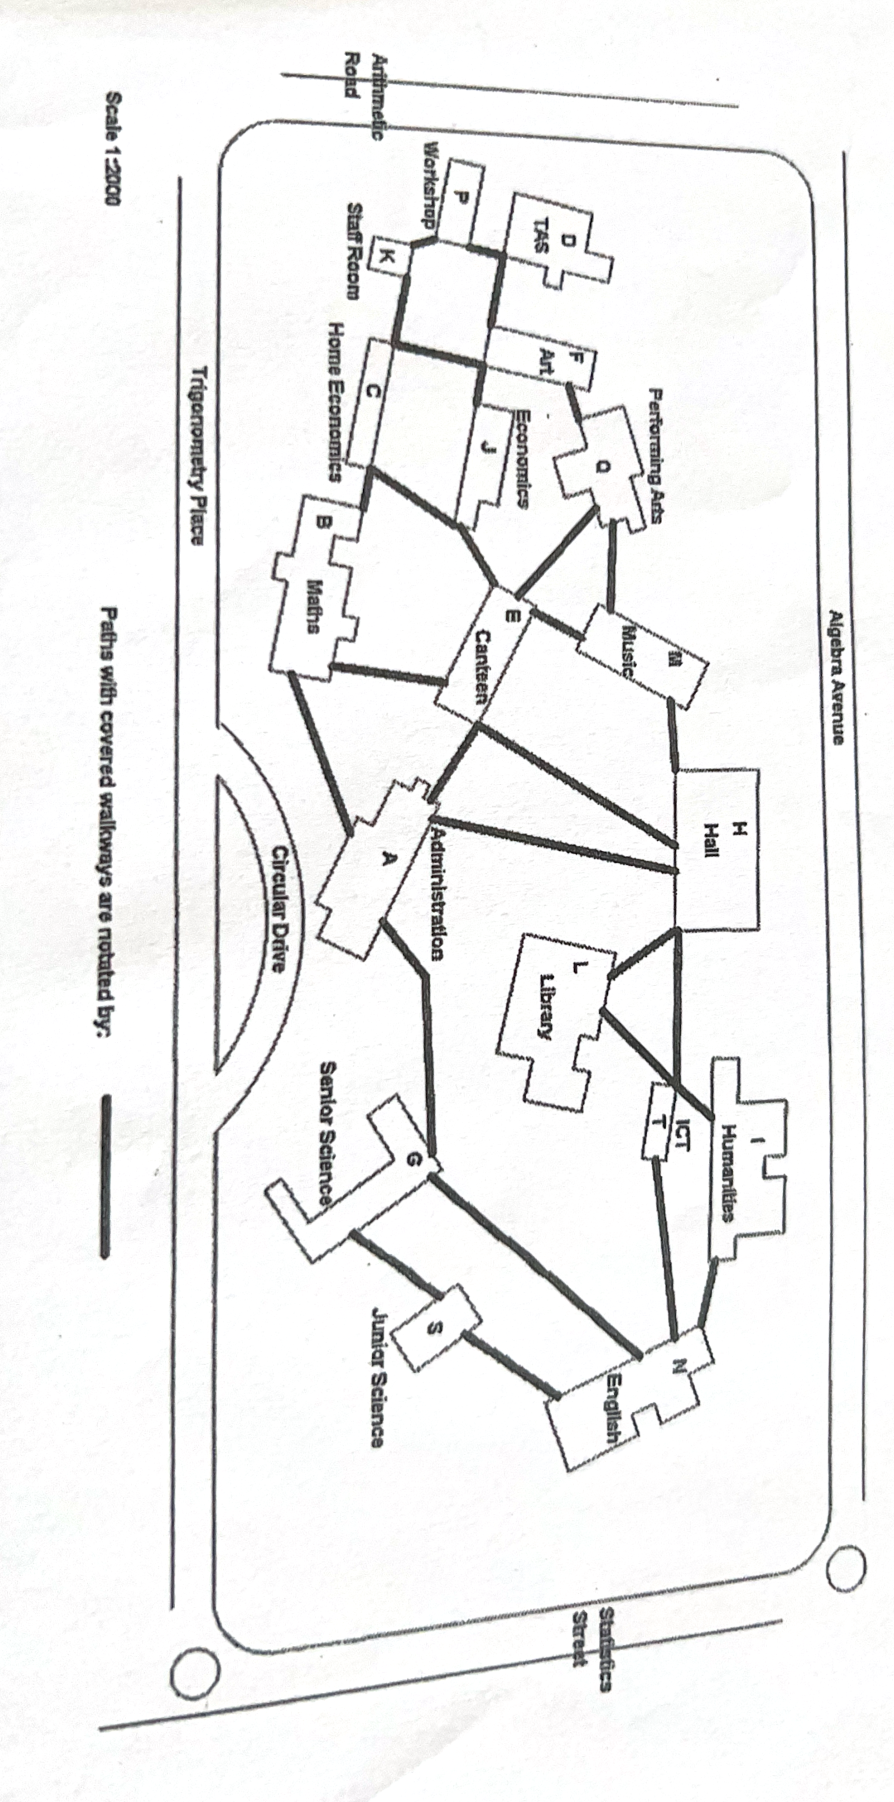
\includegraphics[width=0.5\linewidth]{img/map_orig.png}
    \caption{Inital Floor Plan}
    \label{fig:enter-label}
\end{figure}

\addcontentsline{toc}{subsection}{Converting Map Distance to Real Distance}
\begin{table}[]
\begin{tabular}{lllll}
Node Start & Node Finish & Map Dist (mm) & Actual Dist (m) & Working Out \\
A & B & 17 & 34 & 2000÷1000 x 17 \\
A & E & 9 & 18 & 2000÷1000 x 9 \\
A & G & 18 & 36 & 2000÷1000 x 18 \\
A & H & 26 & 52 & 2000÷1000 x 26 \\
B & C & 4 & 8 & 2000÷1000 x 4 \\
B & E & 17 & 22 & 2000÷1000 x 17 \\
C & F & 9 & 18 & 2000÷1000 x 9 \\
C & J & 11 & 22 & 2000÷1000 x 11 \\
C & K & 7 & 14 & 2000÷1000 x 7 \\
D & F & 7 & 14 & 2000÷1000 x 7 \\
D & P & 3 & 6 & 2000÷1000 x 3 \\
E & J & 7 & 14 & 2000÷1000 x 7 \\
E & M & 6 & 12 & 2000÷1000 x 6 \\
E & Q & 8 & 16 & 2000÷1000 x 8 \\
F & J & 4 & 8 & 2000÷1000 x 4 \\
F & Q & 4 & 8 & 2000÷1000 x 4 \\
G & N & 29 & 58 & 2000÷1000 x 29 \\
G & S & 11 & 22 & 2000÷1000 x 11 \\
H & E & 24 & 48 & 2000÷1000 x 24 \\
H & L & 8 & 16 & 2000÷1000 x 8 \\
H & M & 7 & 14 & 2000÷1000 x 7 \\
H & T & 16 & 32 & 2000÷1000 x 16 \\
I & N & 7 & 14 & 2000÷1000 x 7 \\
I & T & 5 & 10 & 2000÷1000 x 5 \\
K & P & 3 & 6 & 2000÷1000 x 3 \\
L & T & 11 & 22 & 2000÷1000 x 11 \\
M & Q & 9 & 18 & 2000÷1000 x 9 \\
N & S & 12 & 24 & 2000÷1000 x 12 \\
N & T & 18 & 36 & 2000÷1000 x 18 \\
  &   & Total Weight :& 622 &
\end{tabular}
\caption{Full Network Diagram Calculations}
\label{tab:my-table}
\end{table}

\addcontentsline{toc}{subsection}{Redrawn Network Diagram with Actual Distance Weights}
\begin{figure}
    \centering
    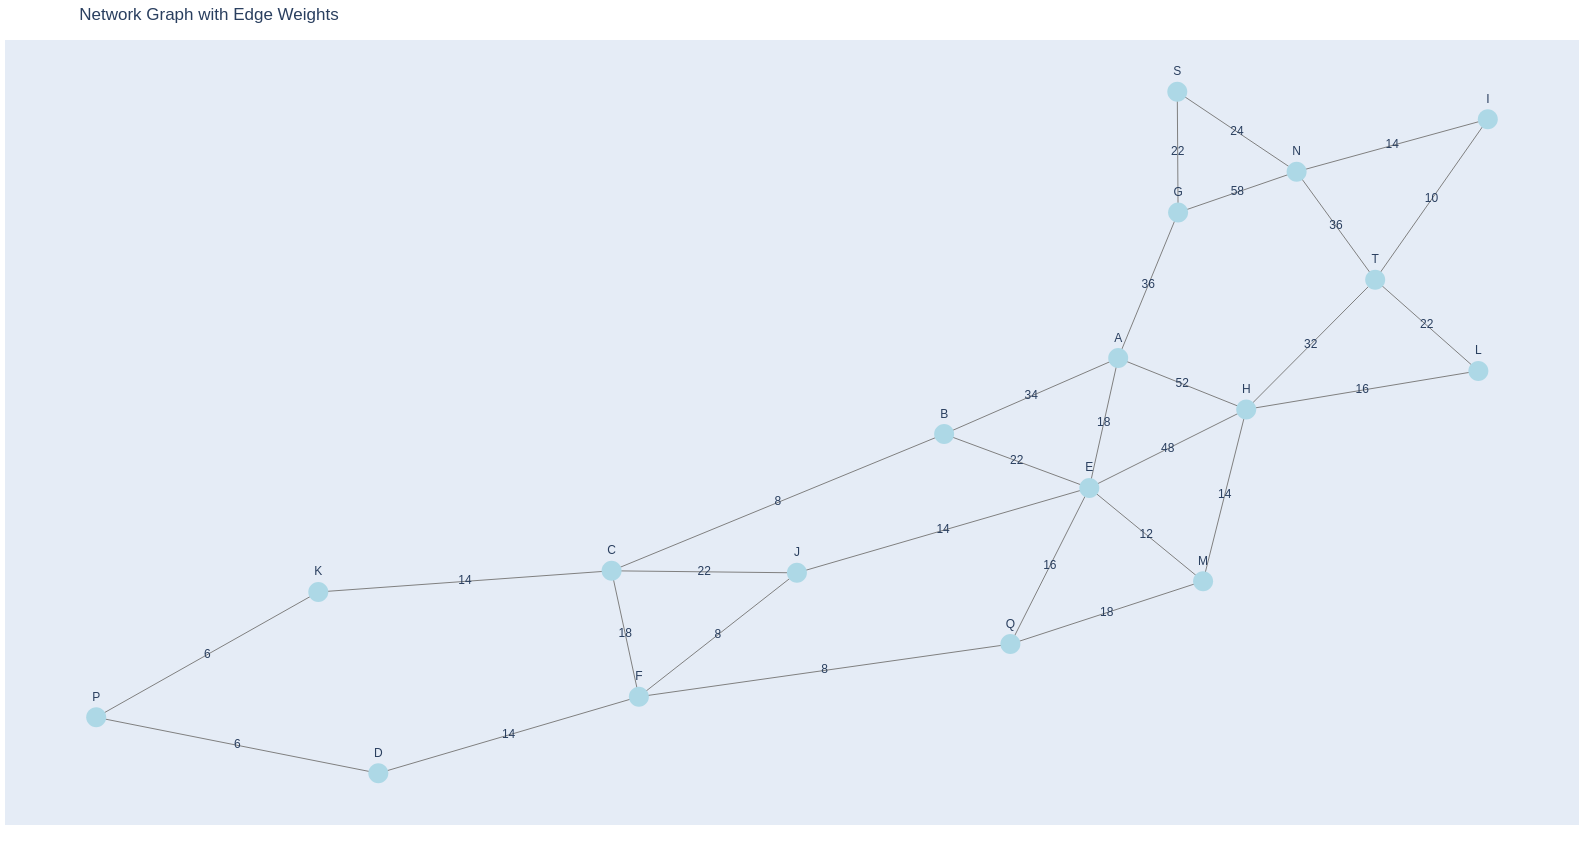
\includegraphics[width=1\linewidth]{img/FullMapWeights.png}
    \caption{Full Network Diagram with Actual Distance Weights}
    \label{fig:enter-label}
\end{figure}

\chapter{Part 2}
The Department of Education wants to link the outside of each building to a computer network. Cable costs \$45 per metre, and the existing walkways are to be used with cabled attached to the roof of the walkways.

Al-Khwaizmi Simple Data (Company A) is asked to submit a proposal.

\section{Al-Khwaizmi Simple Data Quote}
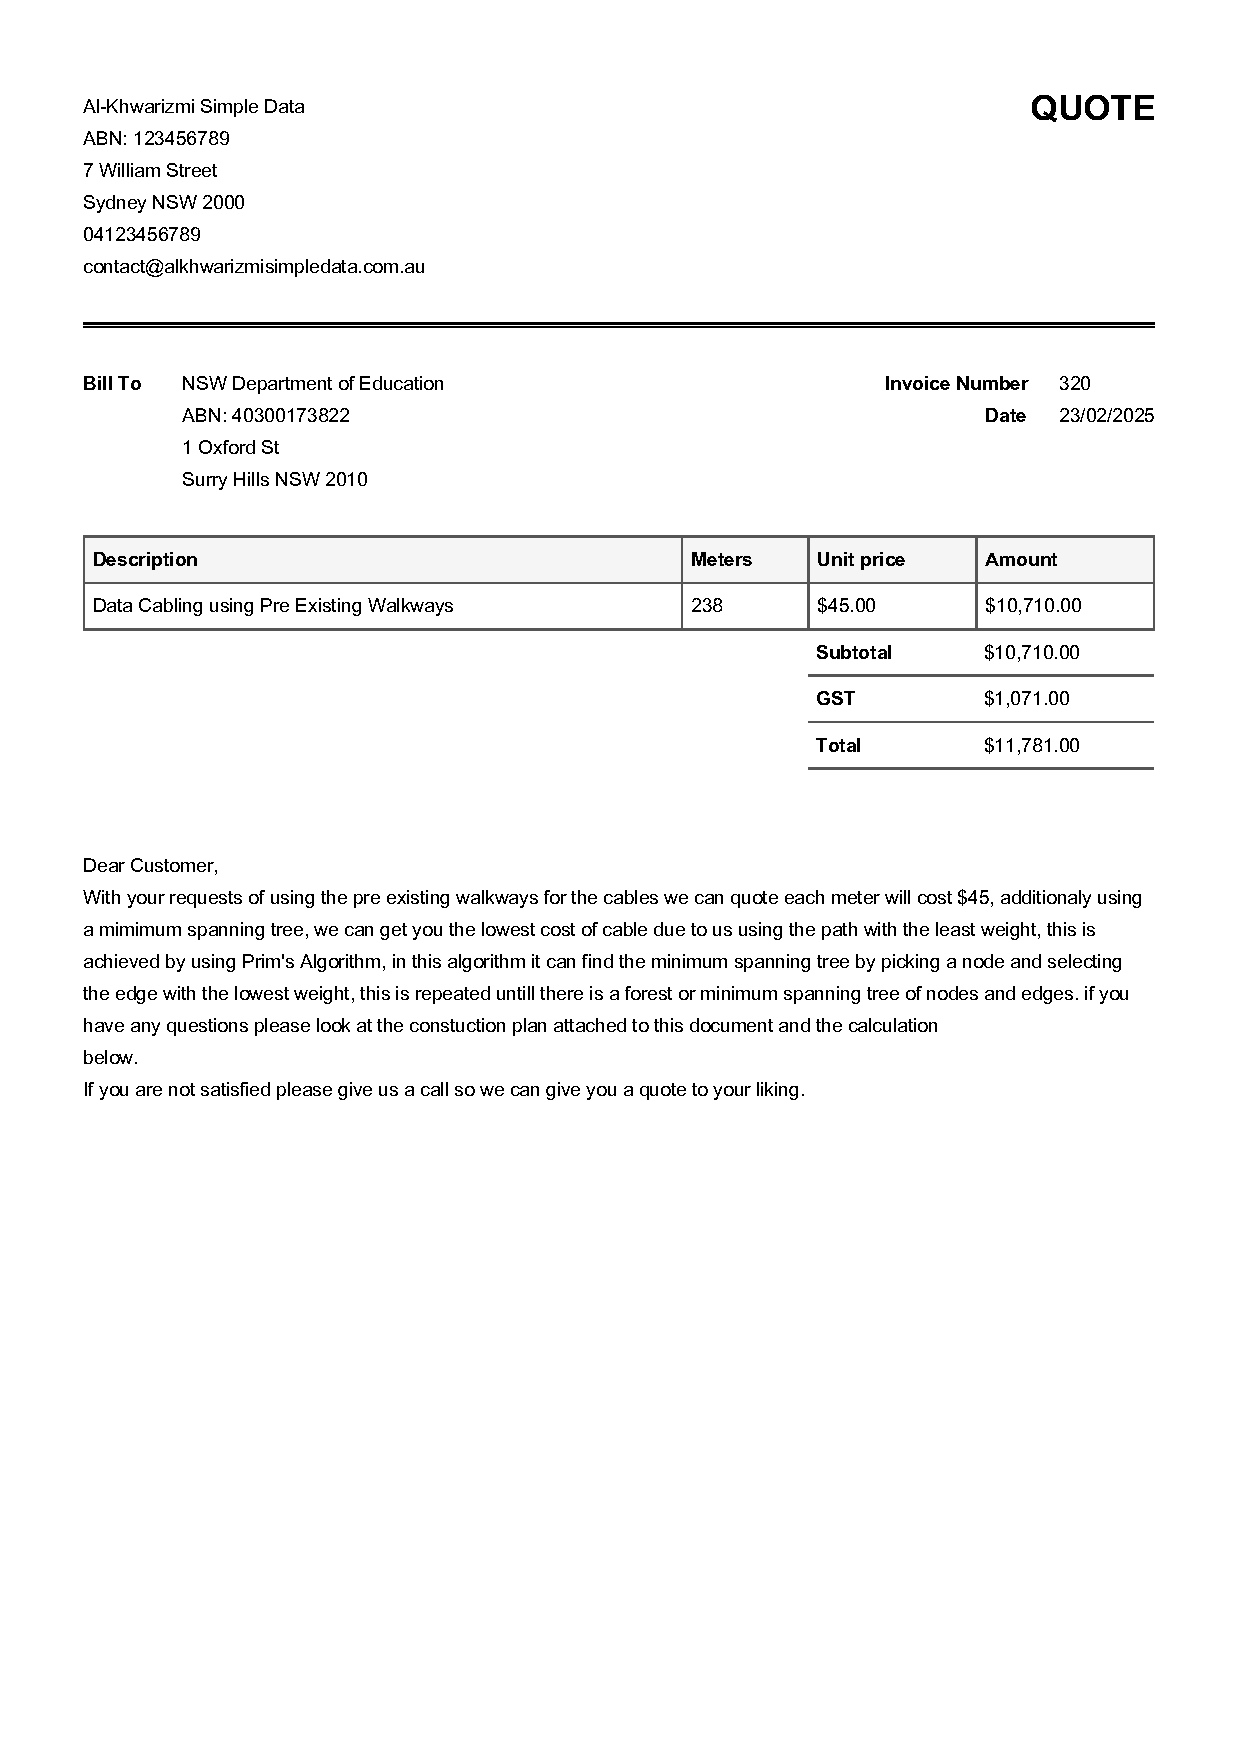
\includepdf[]{pdf/simpdata.pdf}

\section{Al-Khwaizmi Simple Data Construction Plan}
\begin{sidewaysfigure}[ht]
    \centering
    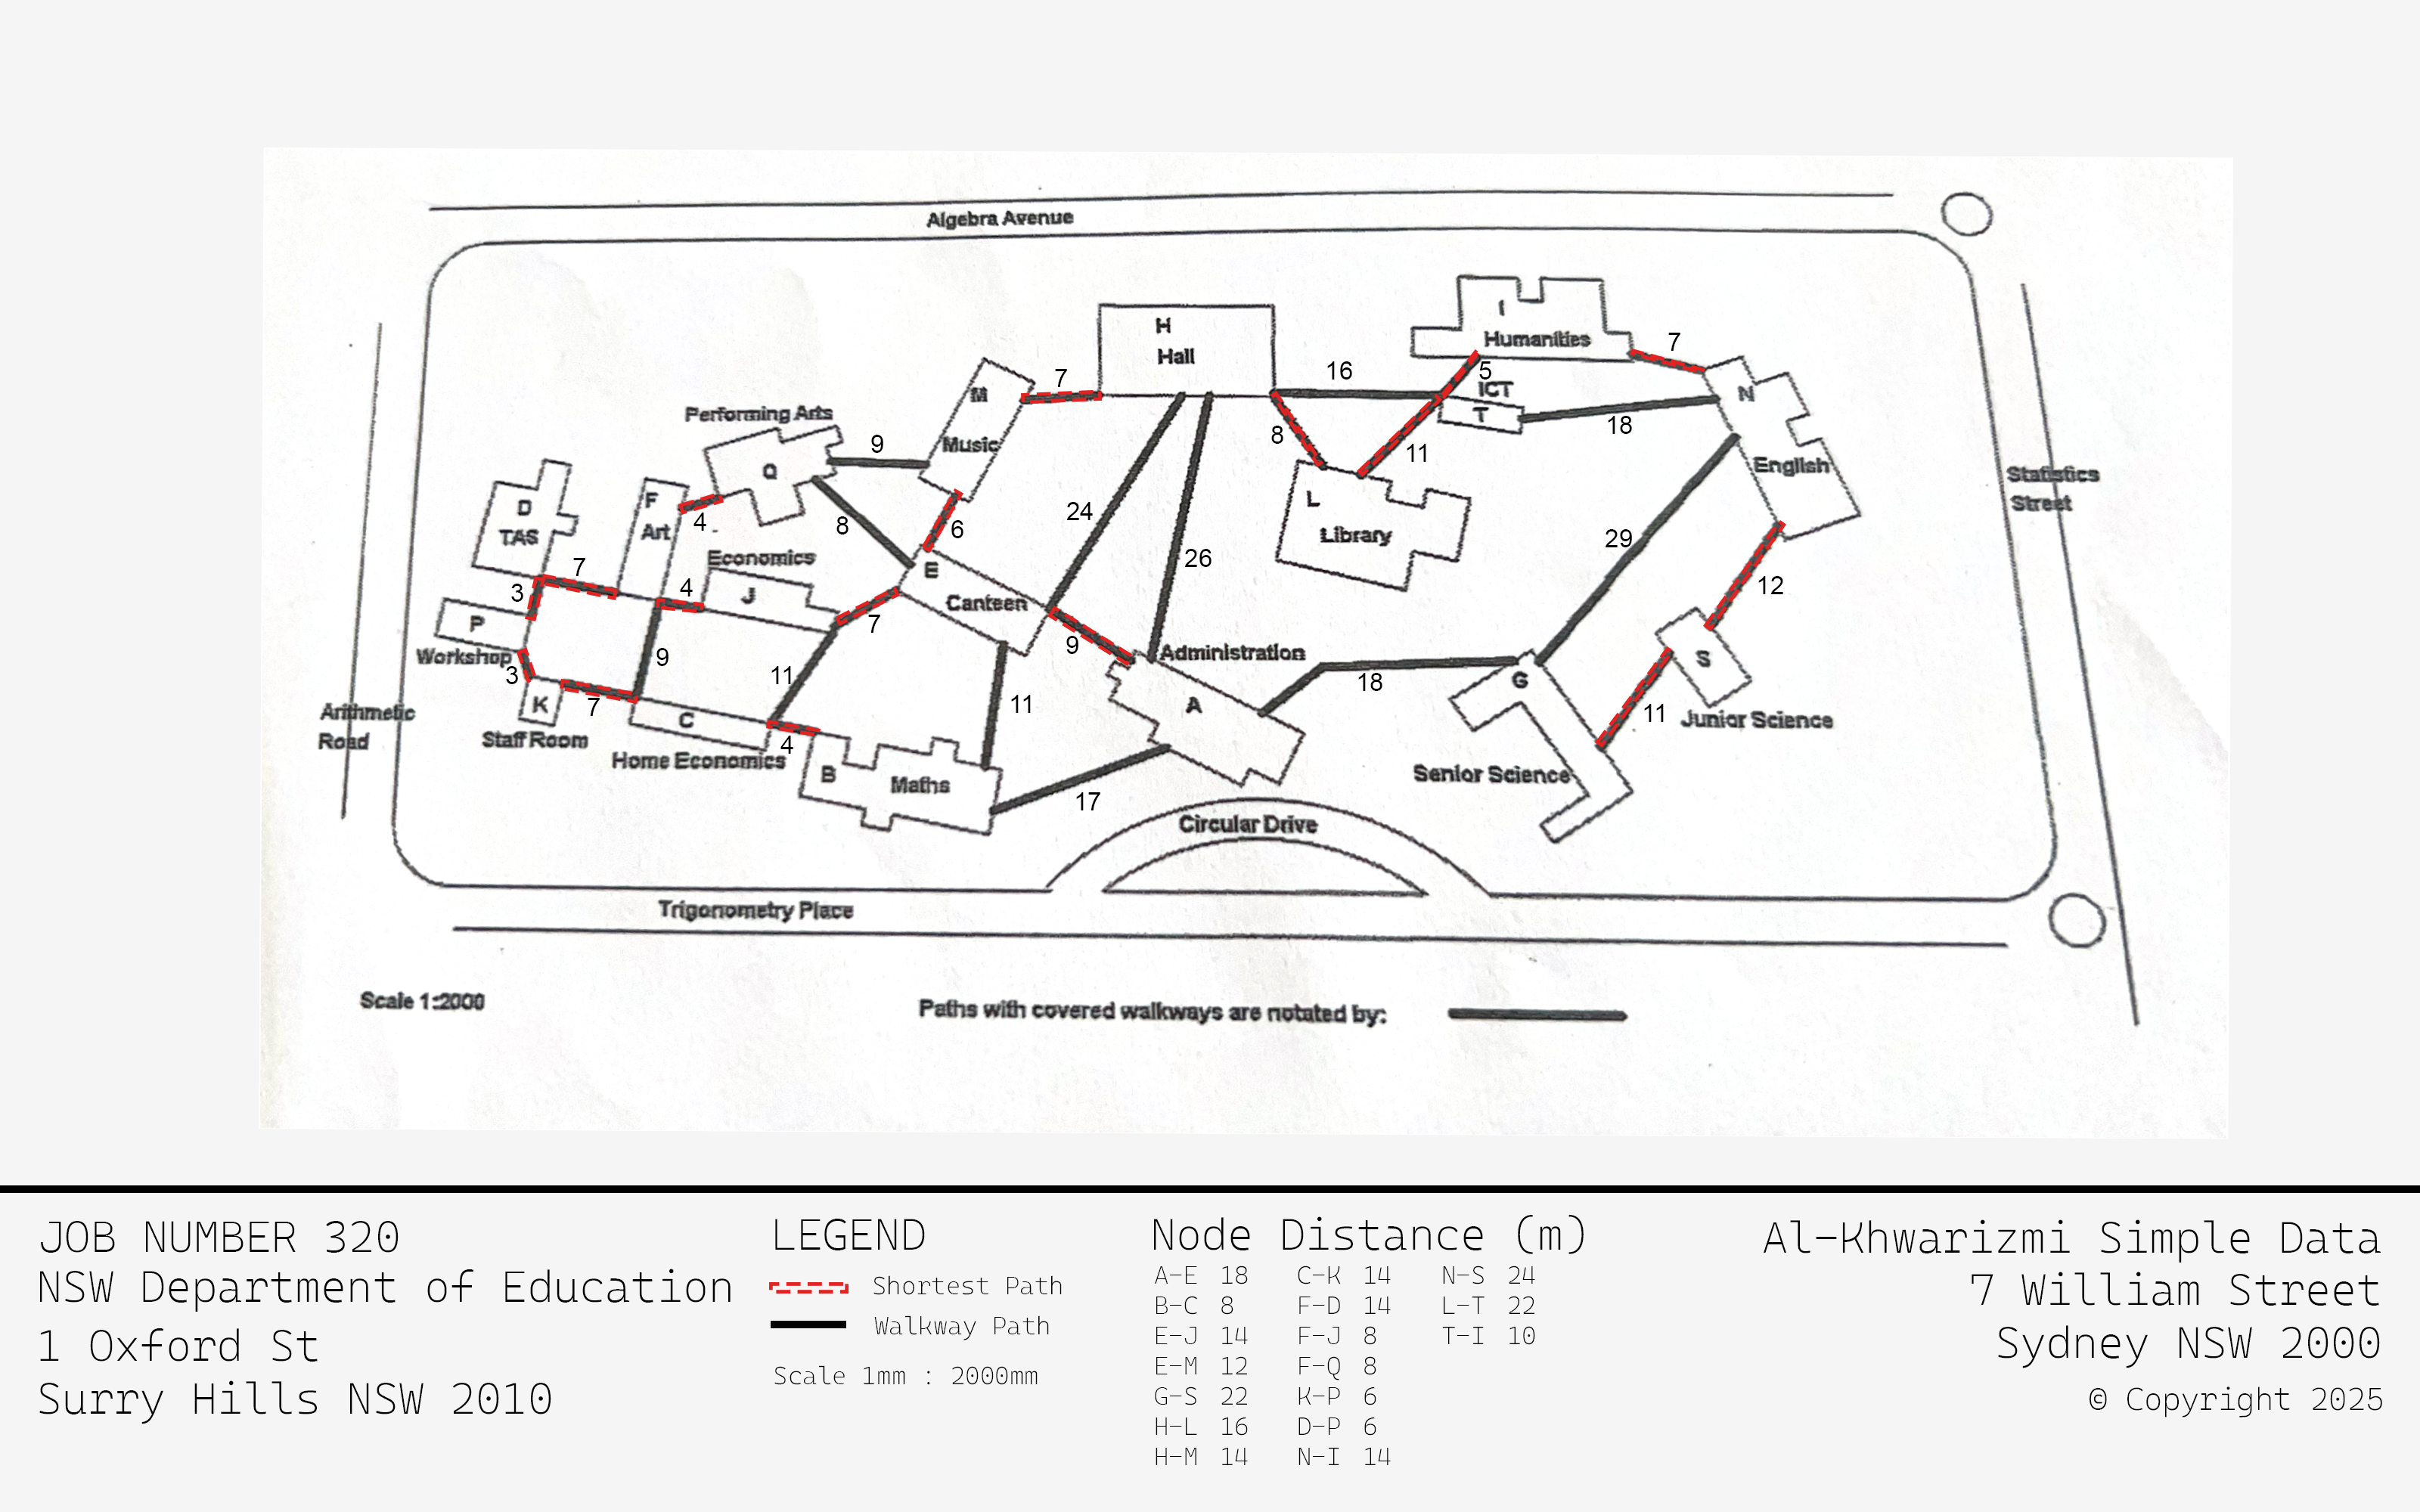
\includegraphics[width=1\linewidth]{img/Al-Khwaizmi Simple Data Plan.png}
    \caption{Al-Khwaizmi Simple Data Construction Plan.}
    \label{fig:enter-label}
\end{sidewaysfigure}

\section{Al-Khwaizmi Simple Data Minimal Spanning Tree}
\begin{sidewaysfigure}[ht]
    \centering
    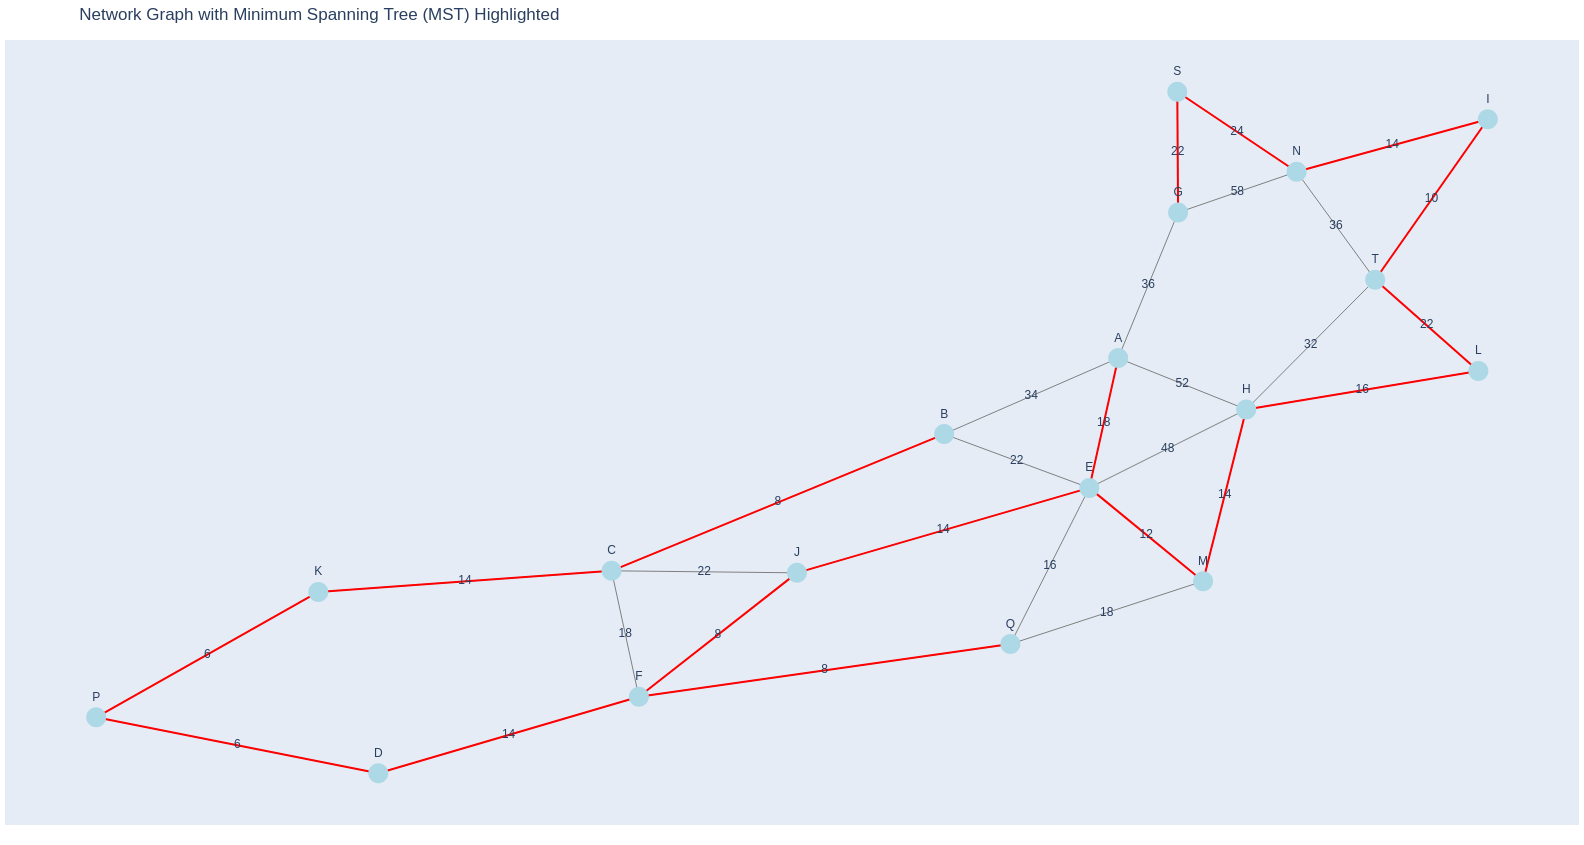
\includegraphics[width=1\linewidth]{img/MST Al-Khwaizmi Simple Data.png}
    \caption{Al-Khwaizmi Simple Data Construction Plan.}
    \label{fig:enter-label}
\end{sidewaysfigure}

\section{Al-Khwaizmi Simple Data Minimal Spanning Tree Calculations}
\begin{table}[]
\begin{tabular}{llllllll}
Step & Start Node & End Node & Weight & Forms Cycle & Is Lowest Edge & Added &  \\
0 & P & - & - & - & - & - &  \\
1 & P & D & 6 & FALSE & TRUE & \cellcolor[HTML]{67FD9A}1 &  \\
2 & P & K & 6 & FALSE & TRUE & \cellcolor[HTML]{67FD9A}1 &  \\
3 & K & C & 14 & FALSE & TRUE & \cellcolor[HTML]{67FD9A}1 &  \\
4 & D & F & 14 & FALSE & TRUE & \cellcolor[HTML]{67FD9A}1 &  \\
5 & F & C & 18 & TRUE & FALSE & \cellcolor[HTML]{FD6864}0 &  \\
6 & F & J & 8 & FALSE & TRUE & \cellcolor[HTML]{67FD9A}1 &  \\
7 & F & Q & 8 & FALSE & TRUE & \cellcolor[HTML]{67FD9A}1 &  \\
8 & C & B & 8 & FALSE & TRUE & \cellcolor[HTML]{67FD9A}1 &  \\
9 & C & J & 22 & TRUE & FALSE & \cellcolor[HTML]{FD6864}0 &  \\
10 & C & F & 18 & TRUE & FALSE & \cellcolor[HTML]{FD6864}0 &  \\
11 & B & A & 34 & FALSE & FALSE & \cellcolor[HTML]{FD6864}0 &  \\
12 & B & E & 22 & FALSE & FALSE & \cellcolor[HTML]{FD6864}0 &  \\
13 & J & E & 14 & FALSE & FALSE & \cellcolor[HTML]{FD6864}0 &  \\
14 & Q & E & 16 & TRUE & FALSE & \cellcolor[HTML]{FD6864}0 &  \\
15 & Q & M & 18 & FALSE & FALSE & \cellcolor[HTML]{FD6864}0 &  \\
16 & A & G & 36 & FALSE & FALSE & \cellcolor[HTML]{FD6864}0 &  \\
17 & A & H & 52 & FALSE & FALSE & \cellcolor[HTML]{FD6864}0 &  \\
18 & E & J & 22 & FALSE & TRUE & \cellcolor[HTML]{67FD9A}1 &  \\
19 & E & A & 18 & FALSE & TRUE & \cellcolor[HTML]{67FD9A}1 &  \\
20 & E & H & 48 & FALSE & FALSE & \cellcolor[HTML]{FD6864}0 &  \\
21 & E & M & 12 & FALSE & TRUE & \cellcolor[HTML]{67FD9A}1 &  \\
22 & M & H & 14 & FALSE & TRUE & \cellcolor[HTML]{67FD9A}1 &  \\
23 & H & T & 32 & FALSE & FALSE & \cellcolor[HTML]{FD6864}0 &  \\
24 & H & L & 16 & FALSE & TRUE & \cellcolor[HTML]{67FD9A}1 &  \\
25 & L & T & 22 & FALSE & TRUE & \cellcolor[HTML]{67FD9A}1 &  \\
26 & T & N & 36 & FALSE & FALSE & \cellcolor[HTML]{FD6864}0 &  \\
27 & T & I & 10 & FALSE & TRUE & \cellcolor[HTML]{67FD9A}1 &  \\
28 & I & N & 14 & FALSE & TRUE & \cellcolor[HTML]{67FD9A}1 &  \\
29 & N & G & 58 & FALSE & FALSE & \cellcolor[HTML]{FD6864}0 &  \\
30 & N & S & 24 & FALSE & TRUE & \cellcolor[HTML]{67FD9A}1 &  \\
31 & S & G & 22 & FALSE & TRUE & \cellcolor[HTML]{67FD9A}1 &  \\
 &  &  &  &  &  &  &  \\
 &  & Total Weight & 238 &  &  &  &  \\
 &  & Total Cost & \$10,710.00 &  &  &  & 
\end{tabular}
\caption{Al-Khwaizmi Simple Data Minimal Spanning Tree Calculations}
\label{tab:my-table}
\end{table}

\begin{figure}
    \centering
    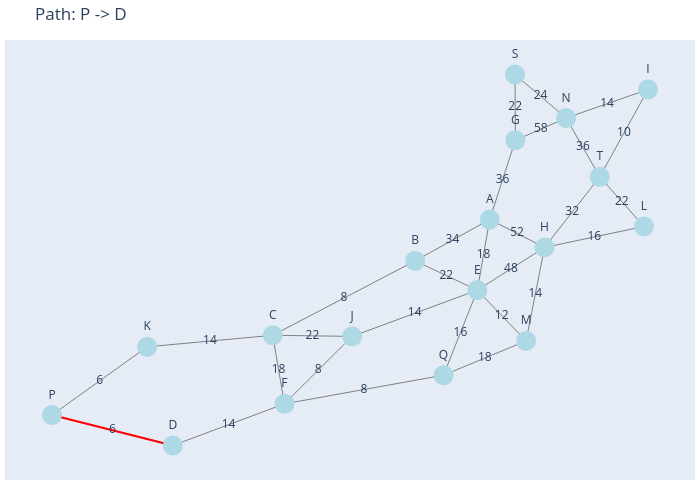
\includegraphics[width=0.7\linewidth]{MSTpath/1.png}
    \caption{P-D}
    \label{fig:enter-label}
\end{figure}
\begin{figure}
    \centering
    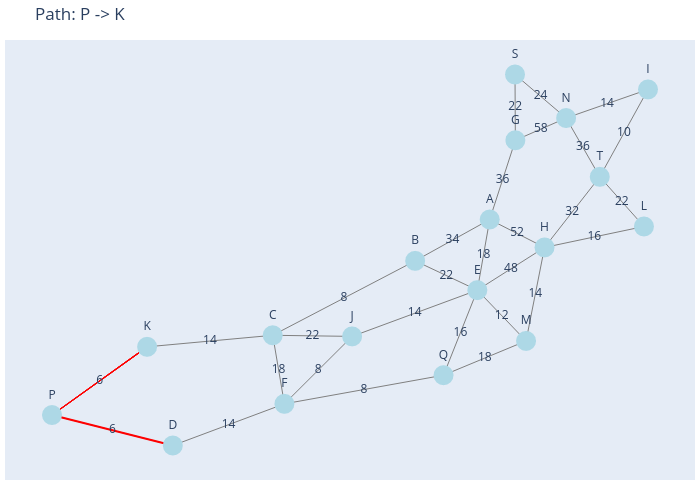
\includegraphics[width=0.7\linewidth]{MSTpath/2.png}
    \caption{P-K}
    \label{fig:enter-label}
\end{figure}
\begin{figure}
    \centering
    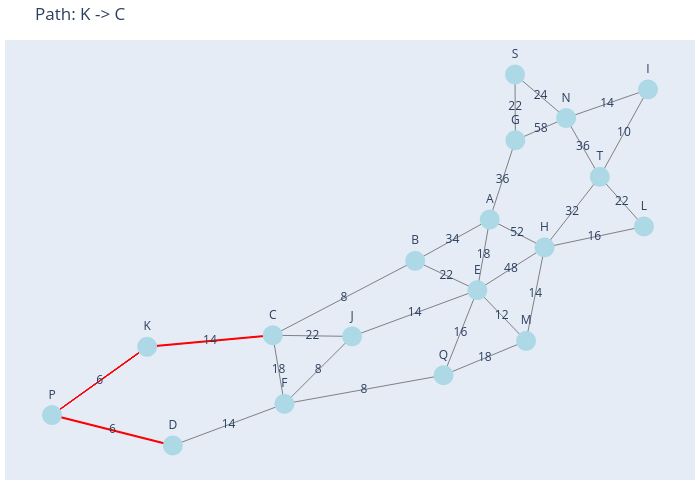
\includegraphics[width=0.7\linewidth]{MSTpath/3.png}
    \caption{K-C}
    \label{fig:enter-label}
\end{figure}
\begin{figure}
    \centering
    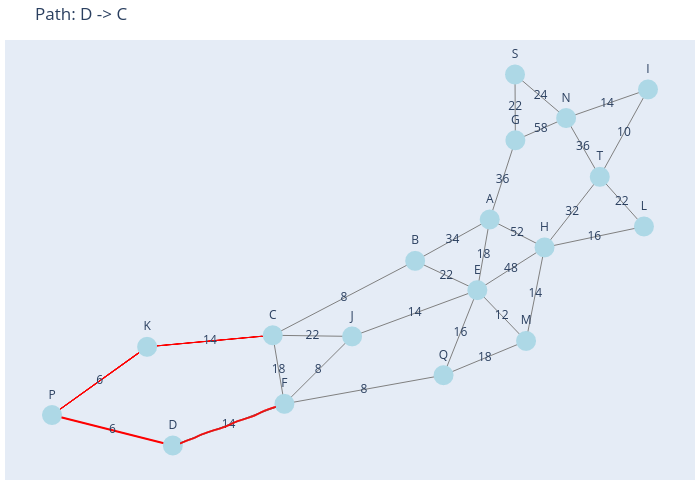
\includegraphics[width=0.7\linewidth]{MSTpath/4.png}
    \caption{D-C}
    \label{fig:enter-label}
\end{figure}
\begin{figure}
    \centering
    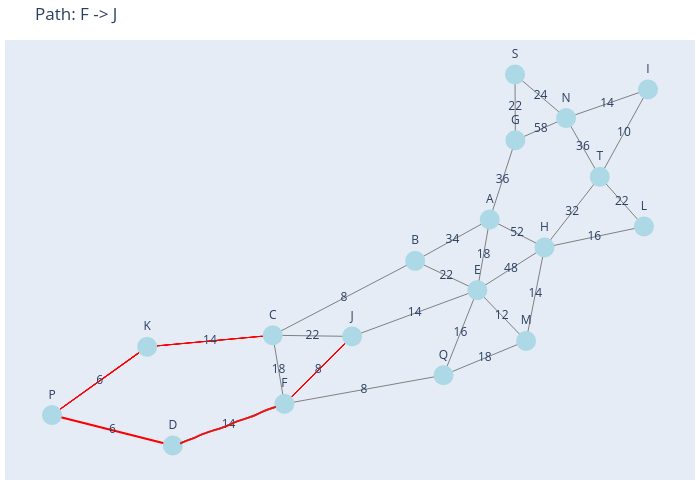
\includegraphics[width=0.7\linewidth]{MSTpath/5.png}
    \caption{F-J}
    \label{fig:enter-label}
\end{figure}
\begin{figure}
    \centering
    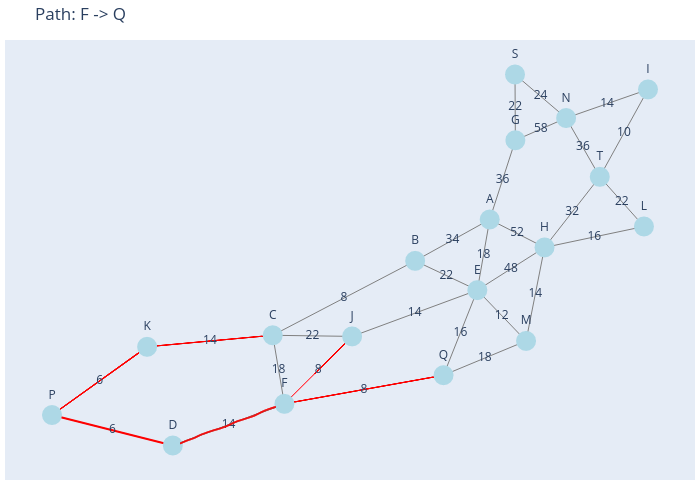
\includegraphics[width=0.7\linewidth]{MSTpath/6.png}
    \caption{F-Q}
    \label{fig:enter-label}
\end{figure}
\begin{figure}
    \centering
    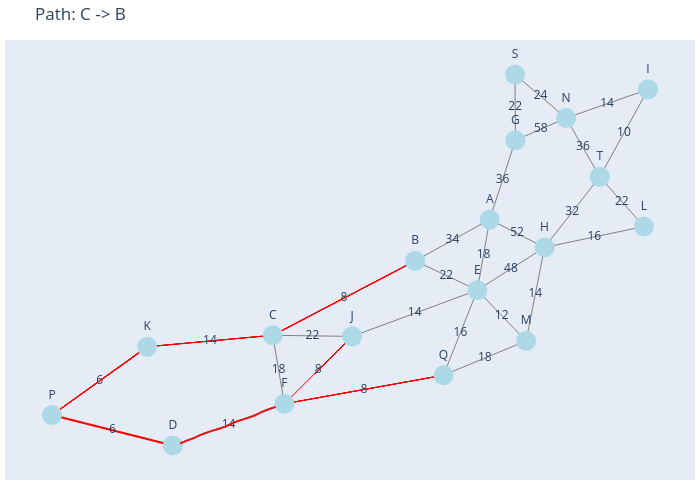
\includegraphics[width=0.7\linewidth]{MSTpath/7.png}
    \caption{C-B}
    \label{fig:enter-label}
\end{figure}
\begin{figure}
    \centering
    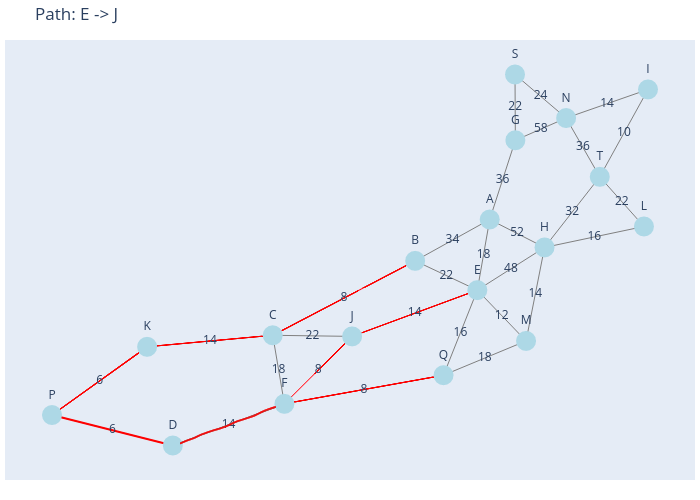
\includegraphics[width=0.7\linewidth]{MSTpath/8.png}
    \caption{E-J}
    \label{fig:enter-label}
\end{figure}
\begin{figure}
    \centering
    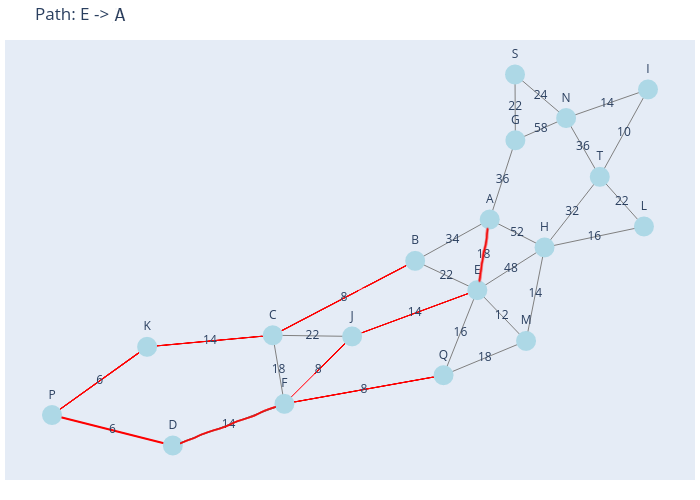
\includegraphics[width=0.7\linewidth]{MSTpath/9.png}
    \caption{E-A}
    \label{fig:enter-label}
\end{figure}
\begin{figure}
    \centering
    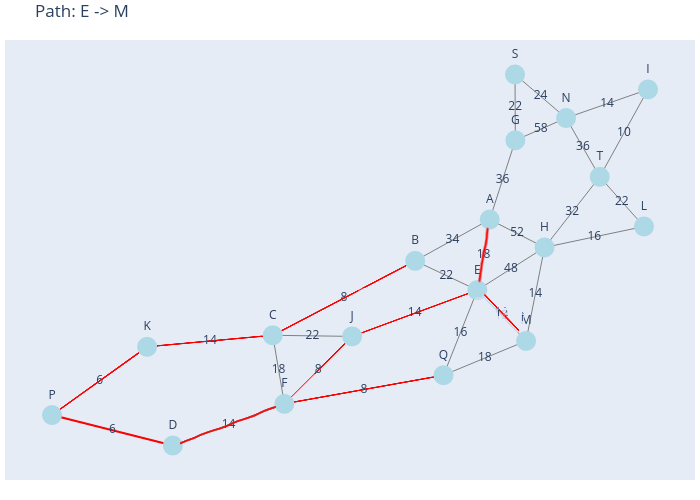
\includegraphics[width=0.7\linewidth]{MSTpath/10.png}
    \caption{E-M}
    \label{fig:enter-label}
\end{figure}
\begin{figure}
    \centering
    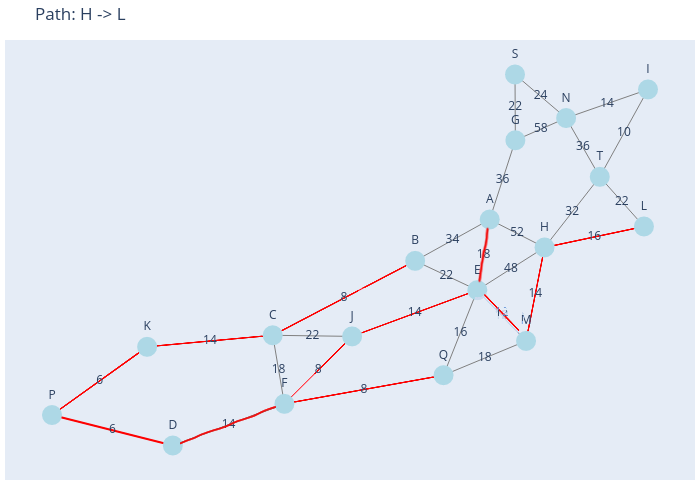
\includegraphics[width=0.7\linewidth]{MSTpath/12.png}
    \caption{H-L}
    \label{fig:enter-label}
\end{figure}
\begin{figure}
    \centering
    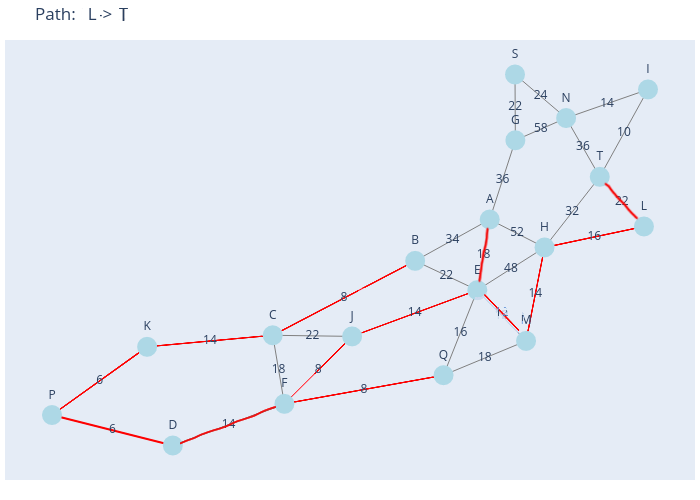
\includegraphics[width=0.7\linewidth]{MSTpath/13.png}
    \caption{L-T}
    \label{fig:enter-label}
\end{figure}
\begin{figure}
    \centering
    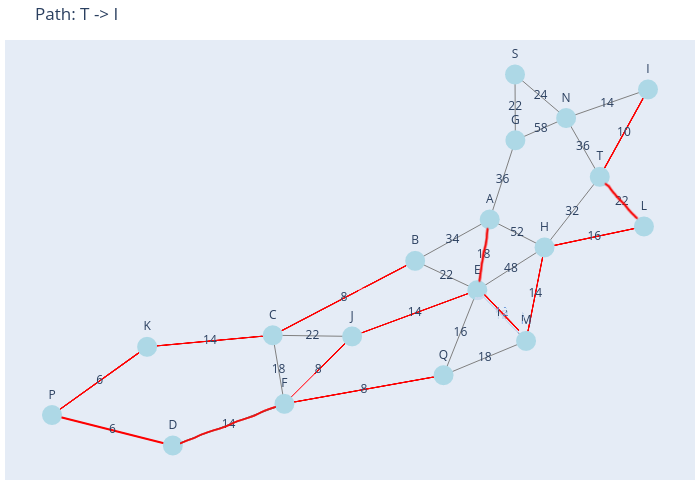
\includegraphics[width=0.7\linewidth]{MSTpath/14.png}
    \caption{T-I}
    \label{fig:enter-label}
\end{figure}
\begin{figure}
    \centering
    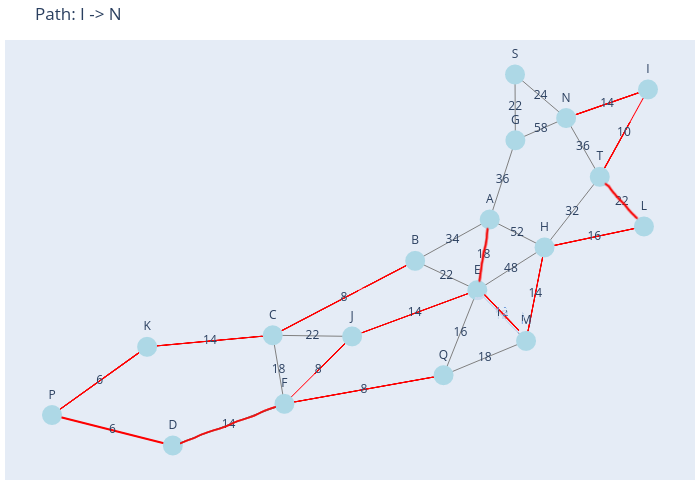
\includegraphics[width=0.7\linewidth]{MSTpath/15.png}
    \caption{I-N}
    \label{fig:enter-label}
\end{figure}
\begin{figure}
    \centering
    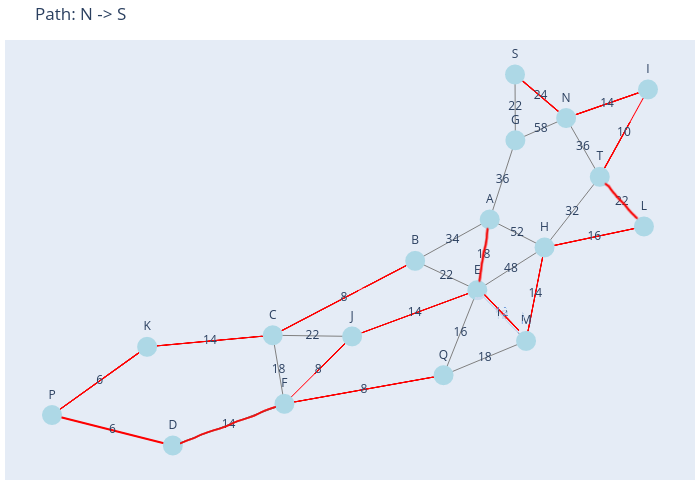
\includegraphics[width=0.7\linewidth]{MSTpath/16.png}
    \caption{N-S}
    \label{fig:enter-label}
\end{figure}
\begin{figure}
    \centering
    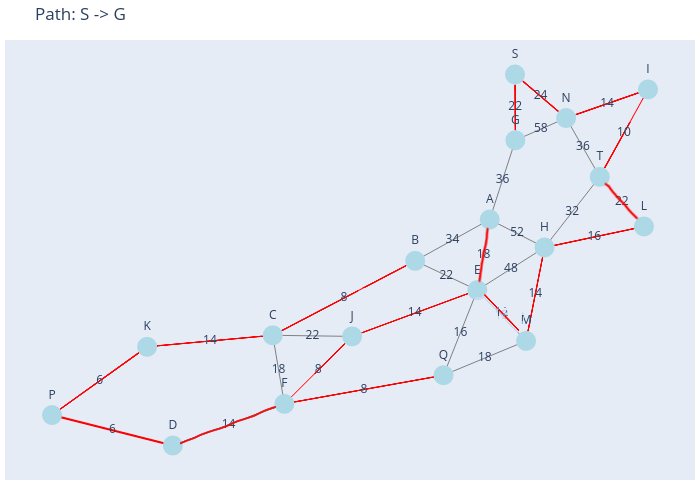
\includegraphics[width=0.7\linewidth]{MSTpath/17.png}
    \caption{S-G}
    \label{fig:enter-label}
\end{figure}


\chapter{Part 3}
In an effort to reduce the costs of cabling the school, the school executive decides that the cable will only run through buildings P and N, connecting only those buildings on the shortest path.
Dijkstra Data (company B) is tasked to submit a proposal to this.

\section{Dijkstra Data Quote}
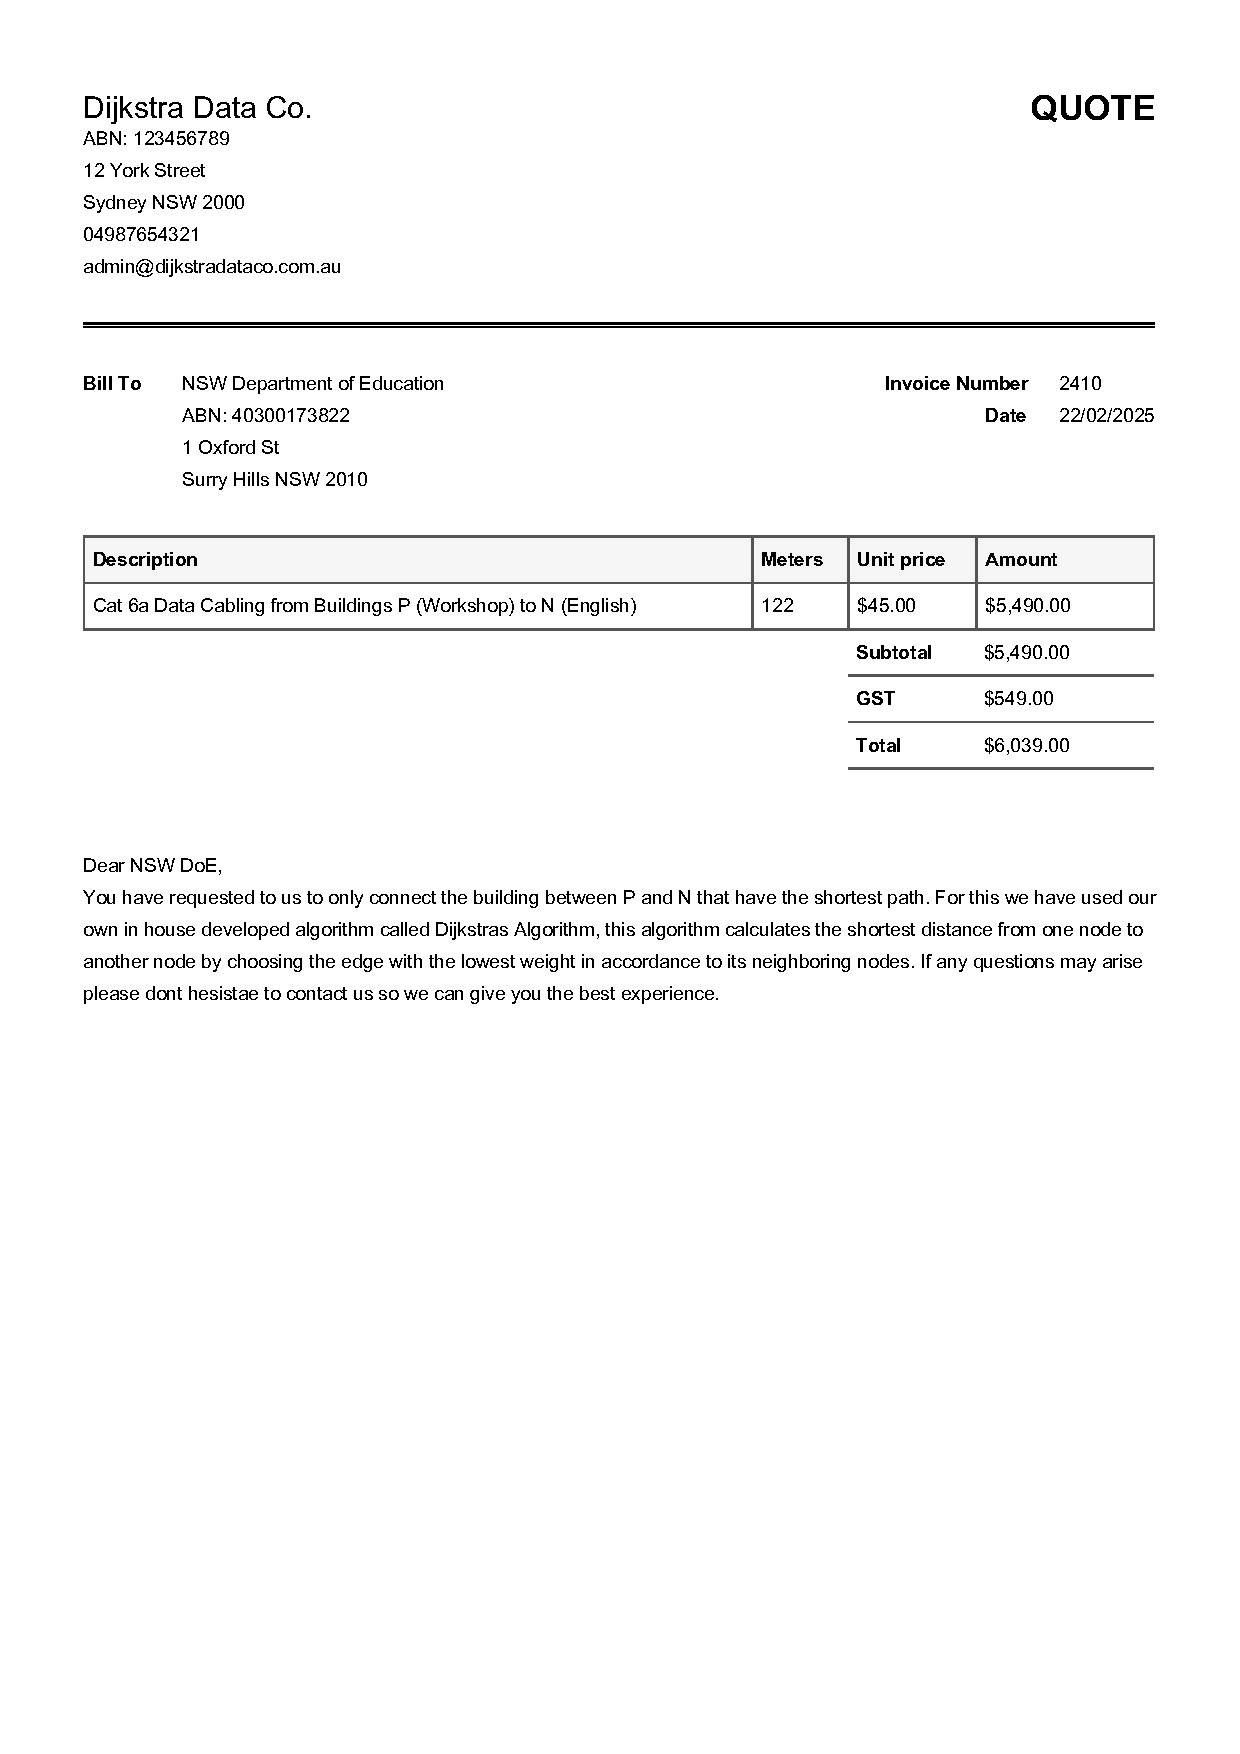
\includepdf[]{pdf/dijkstra.pdf}

\section{Dijkstra Data Construction Plan}
\begin{sidewaysfigure}[ht]
    \centering
    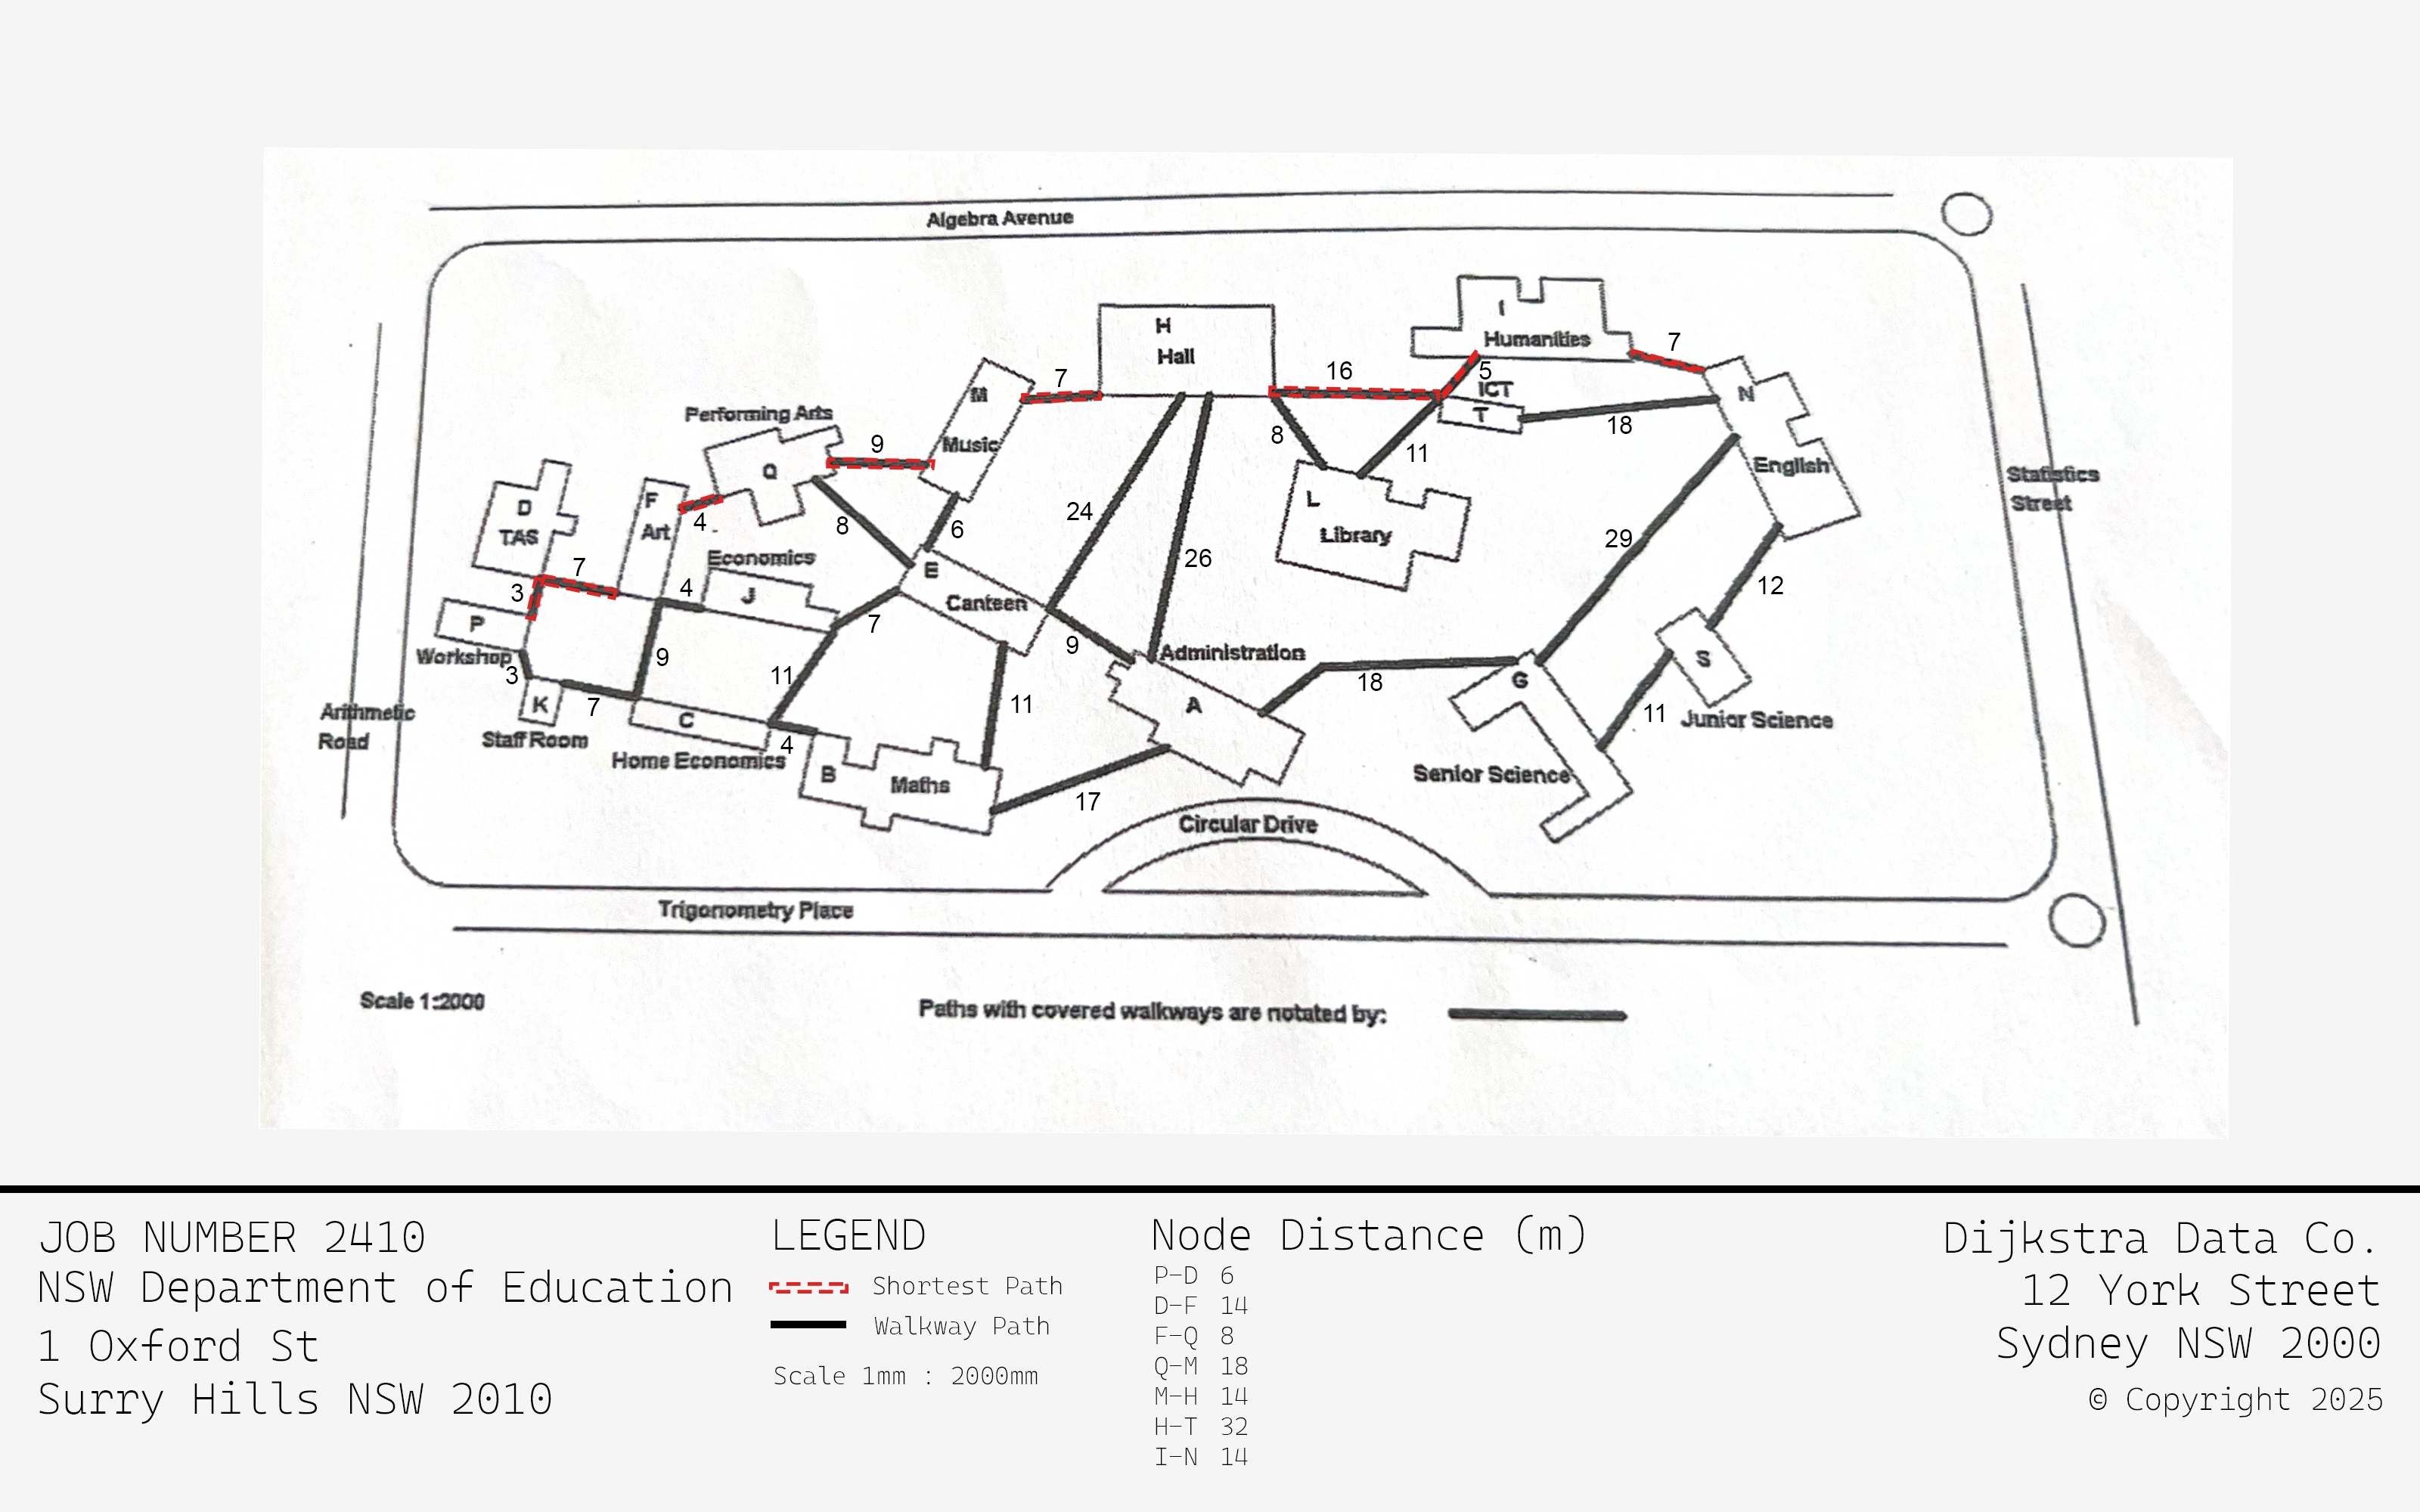
\includegraphics[width=1\linewidth]{img/Dijkstra Data Plan.png}
    \caption{Dijkstra Data Construction Plan.}
    \label{fig:enter-label}
\end{sidewaysfigure}

\section{Dijkstra Data Working Out}
\begin{longtable}{lllllll}
Step & Start & End & Known & Dist to Node & Total Dist & Path \\
\endfirsthead
%
\endhead
%
0 & P & A & FALSE & inf &  &  \\
0 & P & B & FALSE & inf &  &  \\
0 & P & C & FALSE & inf &  &  \\
0 & P & D & TRUE & 6 & 6 & P-D \\
0 & P & E & FALSE & inf &  &  \\
0 & P & F & FALSE & inf &  &  \\
0 & P & G & FALSE & inf &  &  \\
0 & P & H & FALSE & inf &  &  \\
0 & P & I & FALSE & inf &  &  \\
0 & P & J & FALSE & inf &  &  \\
0 & P & K & TRUE & 6 & 6 & P-K \\
0 & P & L & FALSE & inf &  &  \\
0 & P & M & FALSE & inf &  &  \\
0 & P & N & FALSE & inf &  &  \\
0 & P & P & - & - &  &  \\
0 & P & Q & FALSE & inf &  &  \\
0 & P & S & FALSE & inf &  &  \\
0 & P & T & FALSE & inf &  &  \\
 &  &  &  &  &  &  \\
1 & D & A & FALSE & inf &  &  \\
1 & D & B & FALSE & inf &  &  \\
1 & D & C & FALSE & inf &  &  \\
1 & D & D & - & - &  &  \\
1 & D & E & FALSE & inf &  &  \\
1 & D & F & TRUE & 14 & 20 & P-D-F \\
1 & D & G & FALSE & inf &  &  \\
1 & D & H & FALSE & inf &  &  \\
1 & D & I & FALSE & inf &  &  \\
1 & D & J & FALSE & inf &  &  \\
1 & D & K & FALSE & inf &  &  \\
1 & D & L & FALSE & inf &  &  \\
1 & D & M & FALSE & inf &  &  \\
1 & D & N & FALSE & inf &  &  \\
1 & D & P & - & N/A & - & - \\
1 & D & Q & FALSE & inf &  &  \\
1 & D & S & FALSE & inf &  &  \\
1 & D & T & FALSE & inf &  &  \\
 &  &  &  &  &  &  \\
1 & K & A & FALSE & inf &  &  \\
1 & K & B & FALSE & inf &  &  \\
1 & K & C & TRUE & 14 & 20 & P-K-C \\
1 & K & D & FALSE & inf &  &  \\
1 & K & E & FALSE & inf &  &  \\
1 & K & F & FALSE & inf &  &  \\
1 & K & G & FALSE & inf &  &  \\
1 & K & H & FALSE & inf &  &  \\
1 & K & I & FALSE & inf &  &  \\
1 & K & J & FALSE & inf &  &  \\
1 & K & K & FALSE & inf &  &  \\
1 & K & L & FALSE & inf &  &  \\
1 & K & M & FALSE & inf &  &  \\
1 & K & N & FALSE & inf &  &  \\
1 & K & P & 1 & N/A & - & - \\
1 & K & Q & FALSE & inf &  &  \\
1 & K & S & FALSE & inf &  &  \\
1 & K & T & FALSE & inf &  &  \\
 &  &  &  &  &  &  \\
2 & F & A & FALSE & inf &  &  \\
2 & F & B & FALSE & inf &  &  \\
2 & F & C & TRUE & 18 & 38 & P-D-F-C \\
2 & F & D & - & N/A & - & - \\
2 & F & E & FALSE & inf &  &  \\
2 & F & F & FALSE & inf &  &  \\
2 & F & G & FALSE & inf &  &  \\
2 & F & H & FALSE & inf &  &  \\
2 & F & I & FALSE & inf &  &  \\
2 & F & J & TRUE & 8 & 28 & P-D-F-J \\
2 & F & K & FALSE & inf &  &  \\
2 & F & L & FALSE & inf &  &  \\
2 & F & M & FALSE & inf &  &  \\
2 & F & N & FALSE & inf &  &  \\
2 & F & P & FALSE & inf &  &  \\
2 & F & Q & TRUE & 8 & 28 & P-D-F-Q \\
2 & F & S & FALSE & inf &  &  \\
2 & F & T & FALSE & inf &  &  \\
 &  &  &  &  &  &  \\
2 & C & A & FALSE & inf &  &  \\
2 & C & B & TRUE & 8 & 28 & P-K-C-B \\
2 & C & C & FALSE & inf &  &  \\
2 & C & D & FALSE & inf &  &  \\
2 & C & E & FALSE & inf &  &  \\
2 & C & F & TRUE & 18 & 38 & P-K-C-F \\
2 & C & G & FALSE & inf &  &  \\
2 & C & H & FALSE & inf &  &  \\
2 & C & I & FALSE & inf &  &  \\
2 & C & J & TRUE & 22 & 42 & P-K-C-J \\
2 & C & K & - & N/A & - & - \\
2 & C & L & FALSE & inf &  &  \\
2 & C & M & FALSE & inf &  &  \\
2 & C & N & FALSE & inf &  &  \\
2 & C & P & FALSE & inf &  &  \\
2 & C & Q & FALSE & inf &  &  \\
2 & C & S & FALSE & inf &  &  \\
2 & C & T & FALSE & inf &  &  \\
 &  &  &  &  &  &  \\
3 & J & A & FALSE & inf &  &  \\
3 & J & B & FALSE & inf &  &  \\
3 & J & C & FALSE & inf &  &  \\
3 & J & D & FALSE & inf &  &  \\
3 & J & E & TRUE & 14 & 42 & P-D-F-J-E \\
3 & J & F & - & N/A & - & - \\
3 & J & G & FALSE & inf &  &  \\
3 & J & H & FALSE & inf &  &  \\
3 & J & I & FALSE & inf &  &  \\
3 & J & J & FALSE & inf &  &  \\
3 & J & K & FALSE & inf &  &  \\
3 & J & L & FALSE & inf &  &  \\
3 & J & M & FALSE & inf &  &  \\
3 & J & N & FALSE & inf &  &  \\
3 & J & P & FALSE & inf &  &  \\
3 & J & Q & FALSE & inf &  &  \\
3 & J & S & FALSE & inf &  &  \\
3 & J & T & FALSE & inf &  &  \\
 &  &  &  &  &  &  \\
3 & Q & A & FALSE & inf &  &  \\
3 & Q & B & FALSE & inf &  &  \\
3 & Q & C & FALSE & inf &  &  \\
3 & Q & D & FALSE & inf &  &  \\
3 & Q & E & TRUE & 16 & 44 & P-D-F-Q-E \\
3 & Q & F & - & N/A & - & - \\
3 & Q & G & FALSE & inf &  &  \\
3 & Q & H & FALSE & inf &  &  \\
3 & Q & I & FALSE & inf &  &  \\
3 & Q & J & FALSE & inf &  &  \\
3 & Q & K & FALSE & inf &  &  \\
3 & Q & L & FALSE & inf &  &  \\
3 & Q & M & TRUE & 18 & 46 & P-D-F-Q-M \\
3 & Q & N & FALSE & inf &  &  \\
3 & Q & P & FALSE & inf &  &  \\
3 & Q & Q & FALSE & inf &  &  \\
3 & Q & S & FALSE & inf &  &  \\
3 & Q & T & FALSE & inf &  &  \\
 &  &  &  &  &  &  \\
4 & E & A & TRUE & 18 & 60 & P-D-F-J-E-A \\
4 & E & B & TRUE & 22 & 50 & P-D-F-J-E-B \\
4 & E & C & FALSE & inf &  &  \\
4 & E & D & FALSE & inf &  &  \\
4 & E & E & FALSE & inf &  &  \\
4 & E & F & FALSE & inf &  &  \\
4 & E & G & FALSE & inf &  &  \\
4 & E & H & FALSE & inf &  &  \\
4 & E & I & FALSE & inf &  &  \\
4 & E & J & - & N/A & - & - \\
4 & E & K & FALSE & inf &  &  \\
4 & E & L & FALSE & inf &  &  \\
4 & E & M & TRUE & 12 & 54 & P-D-F-J-E-M \\
4 & E & N & FALSE & inf &  &  \\
4 & E & P & FALSE & inf &  &  \\
4 & E & Q & - & N/A & - & - \\
4 & E & S & FALSE & inf &  &  \\
4 & E & T & FALSE & inf &  &  \\
 &  &  &  &  &  &  \\
4 & M & A & FALSE & inf &  &  \\
4 & M & B & FALSE & inf &  &  \\
4 & M & C & FALSE & inf &  &  \\
4 & M & D & FALSE & inf &  &  \\
4 & M & E & - & N/A & - & - \\
4 & M & F & FALSE & inf &  &  \\
4 & M & G & FALSE & inf &  &  \\
4 & M & H & TRUE & 14 & 60 & P-D-F-Q-M-H \\
4 & M & I & FALSE & inf &  &  \\
4 & M & J & FALSE & inf &  &  \\
4 & M & K & FALSE & inf &  &  \\
4 & M & L & FALSE & inf &  &  \\
4 & M & M & FALSE & inf &  &  \\
4 & M & N & FALSE & inf &  &  \\
4 & M & P & FALSE & inf &  &  \\
4 & M & Q & - & N/A & - & - \\
4 & M & S & FALSE & inf &  &  \\
4 & M & T & FALSE & inf &  &  \\
 &  &  &  &  &  &  \\
5 & B & A & TRUE & 34 & 62 & P-K-C-B-A \\
5 & B & B & FALSE & inf &  &  \\
5 & B & C & - & N/A & - & - \\
5 & B & D & FALSE & inf &  &  \\
5 & B & E & - & N/A & - & - \\
5 & B & F & FALSE & inf &  &  \\
5 & B & G & FALSE & inf &  &  \\
5 & B & H & FALSE & inf &  &  \\
5 & B & I & FALSE & inf &  &  \\
5 & B & J & FALSE & inf &  &  \\
5 & B & K & FALSE & inf &  &  \\
5 & B & L & FALSE & inf &  &  \\
5 & B & M & FALSE & inf &  &  \\
5 & B & N & FALSE & inf &  &  \\
5 & B & P & FALSE & inf &  &  \\
5 & B & Q & FALSE & inf &  &  \\
5 & B & S & FALSE & inf &  &  \\
5 & B & T & FALSE & inf &  &  \\
 &  &  &  &  &  &  \\
5 & H & A & TRUE & 52 & 112 & P-D-F-Q-M-H-A \\
5 & H & B & FALSE & inf &  &  \\
5 & H & C & FALSE & inf &  &  \\
5 & H & D & FALSE & inf &  &  \\
5 & H & E & - & N/A & - & - \\
5 & H & F & FALSE & inf &  &  \\
5 & H & G & FALSE & inf &  &  \\
5 & H & H & FALSE & inf &  &  \\
5 & H & I & FALSE & inf &  &  \\
5 & H & J & FALSE & inf &  &  \\
5 & H & K & FALSE & inf &  &  \\
5 & H & L & TRUE & 16 & 76 & P-D-F-Q-M-H-L \\
5 & H & M & - & N/A & - & - \\
5 & H & N & FALSE & inf &  &  \\
5 & H & P & FALSE & inf &  &  \\
5 & H & Q & FALSE & inf &  &  \\
5 & H & S & FALSE & inf &  &  \\
5 & H & T & TRUE & 32 & 92 & P-D-F-Q-M-H-T \\
 &  &  &  &  &  &  \\
6 & L & A & FALSE & inf &  &  \\
6 & L & B & FALSE & inf &  &  \\
6 & L & C & FALSE & inf &  &  \\
6 & L & D & FALSE & inf &  &  \\
6 & L & E & FALSE & inf &  &  \\
6 & L & F & FALSE & inf &  &  \\
6 & L & G & FALSE & inf &  &  \\
6 & L & H & - & N/A & - & - \\
6 & L & I & FALSE & inf &  &  \\
6 & L & J & FALSE & inf &  &  \\
6 & L & K & FALSE & inf &  &  \\
6 & L & L & FALSE & inf &  &  \\
6 & L & M & FALSE & inf &  &  \\
6 & L & N & FALSE & inf &  &  \\
6 & L & P & FALSE & inf &  &  \\
6 & L & Q & FALSE & inf &  &  \\
6 & L & S & FALSE & inf &  &  \\
6 & L & T & TRUE & 22 & 98 & P-D-F-Q-M-H-L-T \\
 &  &  &  &  &  &  \\
6 & T & A & FALSE & inf &  &  \\
6 & T & B & FALSE & inf &  &  \\
6 & T & C & FALSE & inf &  &  \\
6 & T & D & FALSE & inf &  &  \\
6 & T & E & FALSE & inf &  &  \\
6 & T & F & FALSE & inf &  &  \\
6 & T & G & FALSE & inf &  &  \\
6 & T & H & - & N/A & - & - \\
6 & T & I & TRUE & 10 & 108 & P-D-F-Q-M-H-T-I \\
6 & T & J & FALSE & inf &  &  \\
6 & T & K & FALSE & inf &  &  \\
6 & T & L & - & N/A & - & - \\
6 & T & M & FALSE & inf &  &  \\
6 & T & N & TRUE & 36 & 128 & P-D-F-Q-M-H-T-N \\
6 & T & P & FALSE & inf &  &  \\
6 & T & Q & FALSE & inf &  &  \\
6 & T & S & FALSE & inf &  &  \\
6 & T & T & FALSE & inf &  &  \\
 &  &  &  &  &  &  \\
7 & I & A & FALSE & inf &  &  \\
7 & I & B & FALSE & inf &  &  \\
7 & I & C & FALSE & inf &  &  \\
7 & I & D & FALSE & inf &  &  \\
7 & I & E & FALSE & inf &  &  \\
7 & I & F & FALSE & inf &  &  \\
7 & I & G & FALSE & inf &  &  \\
7 & I & H & FALSE & inf &  &  \\
7 & I & I & FALSE & inf &  &  \\
7 & I & J & FALSE & inf &  &  \\
7 & I & K & FALSE & inf &  &  \\
7 & I & L & FALSE & inf &  &  \\
7 & I & M & FALSE & inf &  &  \\
7 & I & N & TRUE & 14 & \cellcolor[HTML]{67FD9A} 122 & \cellcolor[HTML]{67FD9A} P-D-F-Q-M-H-T-I-N \\
7 & I & P & FALSE & inf &  &  \\
7 & I & Q & FALSE & inf &  &  \\
7 & I & S & FALSE & inf &  &  \\
7 & I & T & - & N/A & - & - \\
 &  &  &  &  &  &  \\
7 & N & A & FALSE & inf &  &  \\
7 & N & B & FALSE & inf &  &  \\
7 & N & C & FALSE & inf &  &  \\
7 & N & D & FALSE & inf &  &  \\
7 & N & E & FALSE & inf &  &  \\
7 & N & F & FALSE & inf &  &  \\
7 & N & G & TRUE & 58 & 180 & P-D-F-Q-M-H-T-N-G \\
7 & N & H & FALSE & inf &  &  \\
7 & N & I & - & N/A & - & - \\
7 & N & J & FALSE & inf &  &  \\
7 & N & K & FALSE & inf &  &  \\
7 & N & L & FALSE & inf &  &  \\
7 & N & M & FALSE & inf &  &  \\
7 & N & N & FALSE & inf &  &  \\
7 & N & P & FALSE & inf &  &  \\
7 & N & Q & FALSE & inf &  &  \\
7 & N & S & TRUE & 24 & 152 & P-D-F-Q-M-H-T-N-S \\
7 & N & T & - & N/A & - & -
\end{longtable}

\begin{figure}
    \centering
    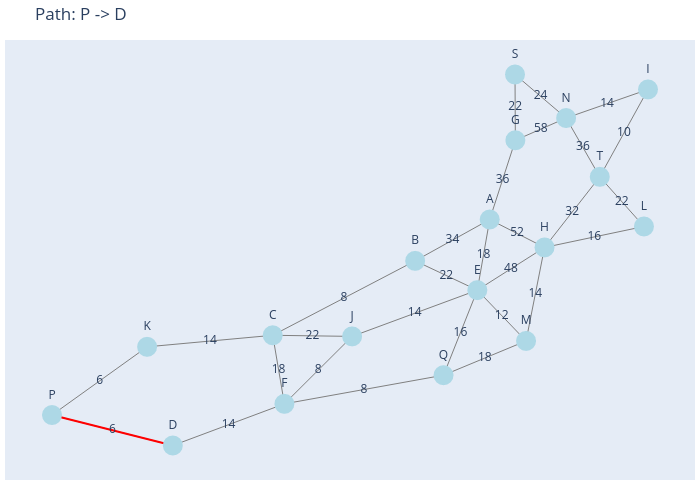
\includegraphics[width=0.7\linewidth]{Plots/P_D.png}
    \caption{P-D}
    \label{fig:enter-label}
\end{figure}
\begin{figure}
    \centering
    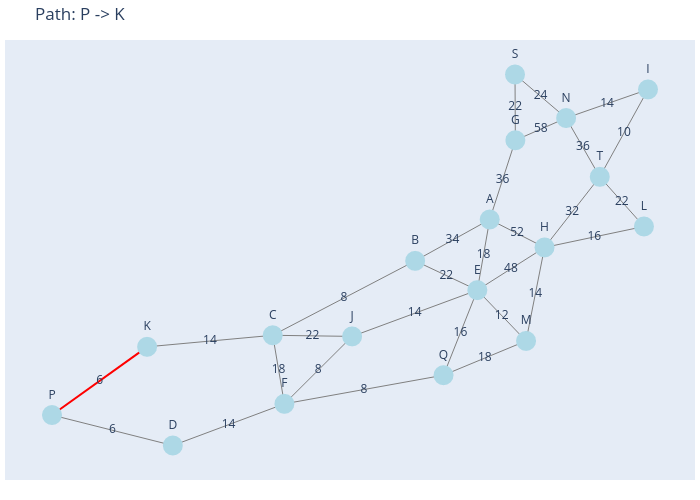
\includegraphics[width=0.7\linewidth]{Plots/P_K.png}
    \caption{P-K}
    \label{fig:enter-label}
\end{figure}
\begin{figure}
    \centering
    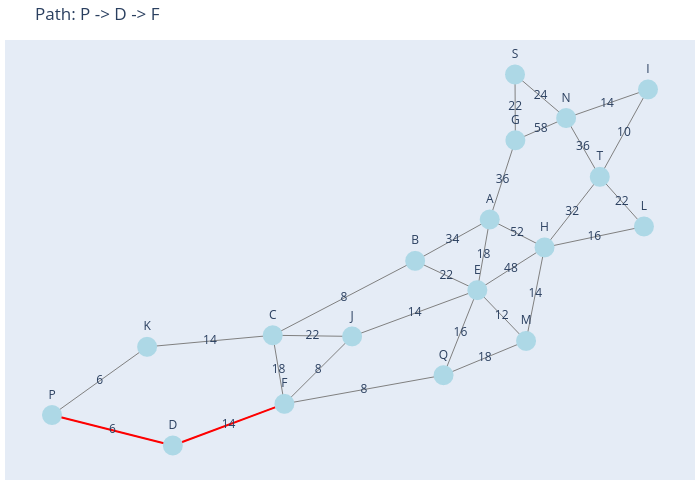
\includegraphics[width=0.7\linewidth]{Plots/P_D_F.png}
    \caption{P-D-F}
    \label{fig:enter-label}
\end{figure}
\begin{figure}
    \centering
    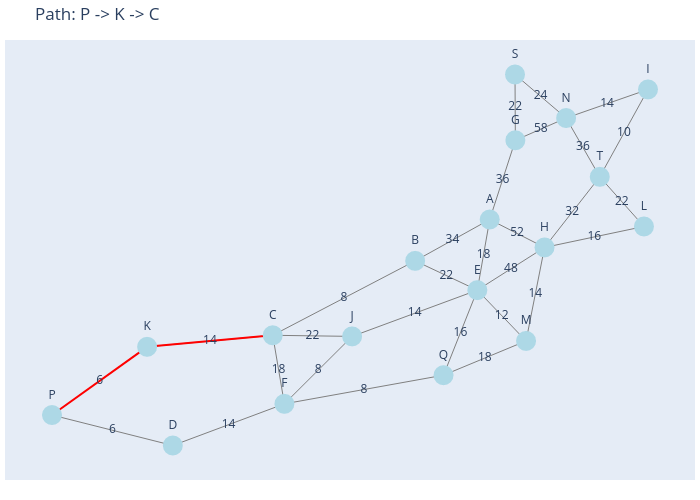
\includegraphics[width=0.7\linewidth]{Plots/P_K_C.png}
    \caption{P-K-C}
    \label{fig:enter-label}
\end{figure}
\begin{figure}
    \centering
    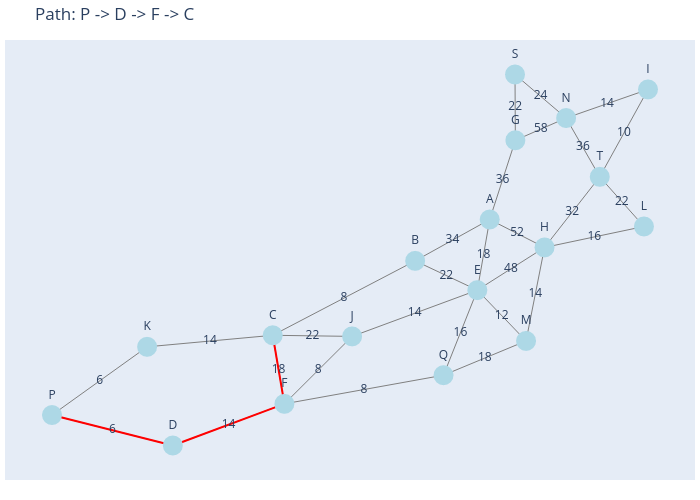
\includegraphics[width=0.7\linewidth]{Plots/P_D_F_C.png}
    \caption{P-D-F-C}
    \label{fig:enter-label}
\end{figure}
\begin{figure}
    \centering
    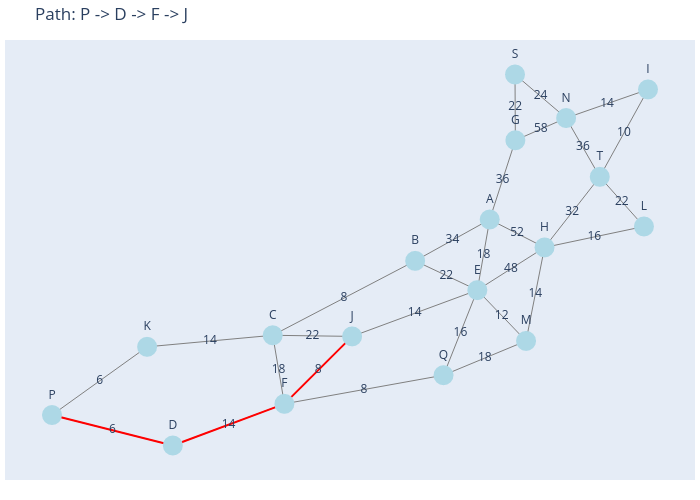
\includegraphics[width=0.7\linewidth]{Plots/P_D_F_J.png}
    \caption{P-D-F-J}
    \label{fig:enter-label}
\end{figure}
\begin{figure}
    \centering
    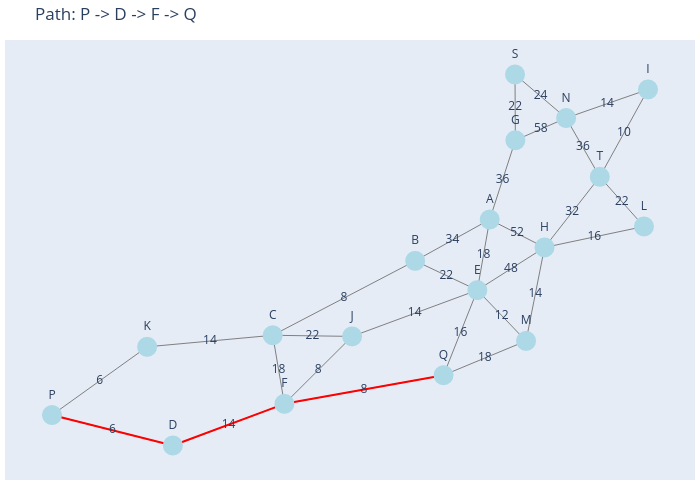
\includegraphics[width=0.7\linewidth]{Plots/P_D_F_Q.png}
    \caption{P-D-F-Q}
    \label{fig:enter-label}
\end{figure}
\begin{figure}
    \centering
    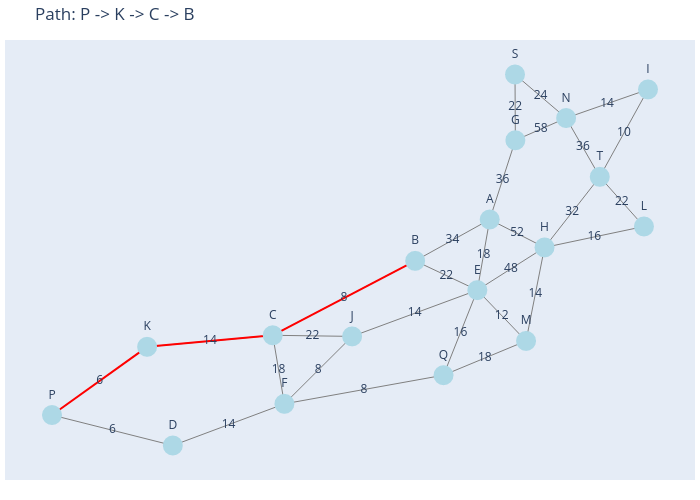
\includegraphics[width=0.7\linewidth]{Plots/P_K_C_B.png}
    \caption{P-K-C-B}
    \label{fig:enter-label}
\end{figure}
\begin{figure}
    \centering
    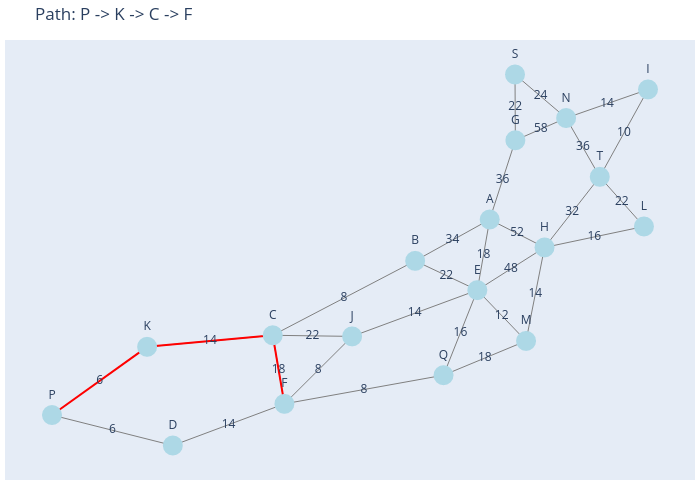
\includegraphics[width=0.7\linewidth]{Plots/P_K_C_F.png}
    \caption{P-K-C-F}
    \label{fig:enter-label}
\end{figure}
\begin{figure}
    \centering
    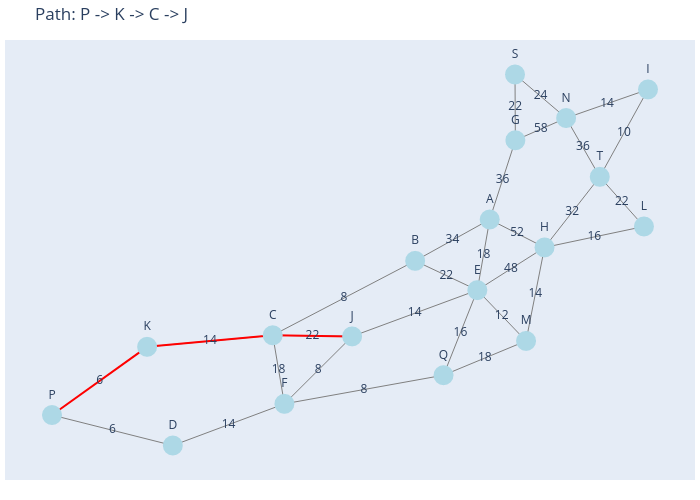
\includegraphics[width=0.7\linewidth]{Plots/P_K_C_J.png}
    \caption{P-K-C-J}
    \label{fig:enter-label}
\end{figure}
\begin{figure}
    \centering
    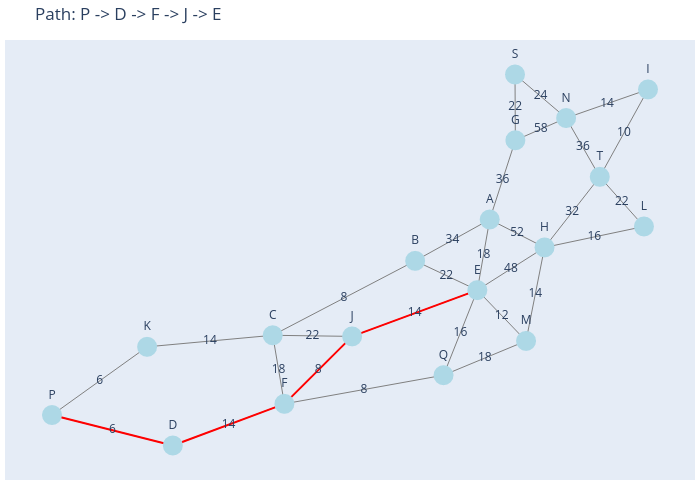
\includegraphics[width=0.7\linewidth]{Plots/P_D_F_J_E.png}
    \caption{P-D-F-J-E}
    \label{fig:enter-label}
\end{figure}
\begin{figure}
    \centering
    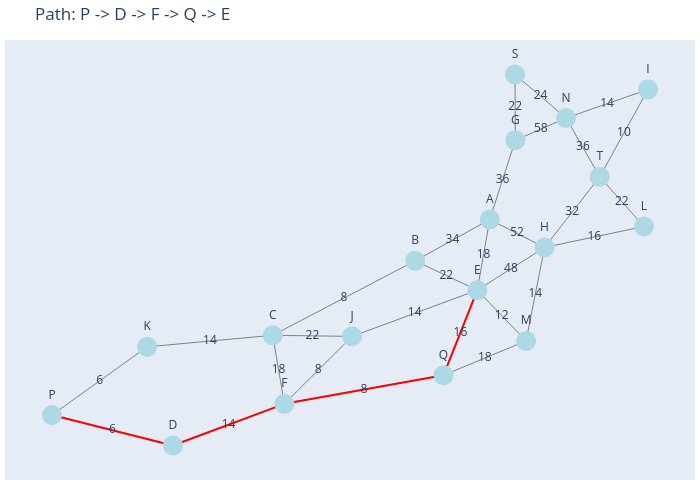
\includegraphics[width=0.7\linewidth]{Plots/P_D_F_Q_E.png}
    \caption{P-D-F-Q-E}
    \label{fig:enter-label}
\end{figure}
\begin{figure}
    \centering
    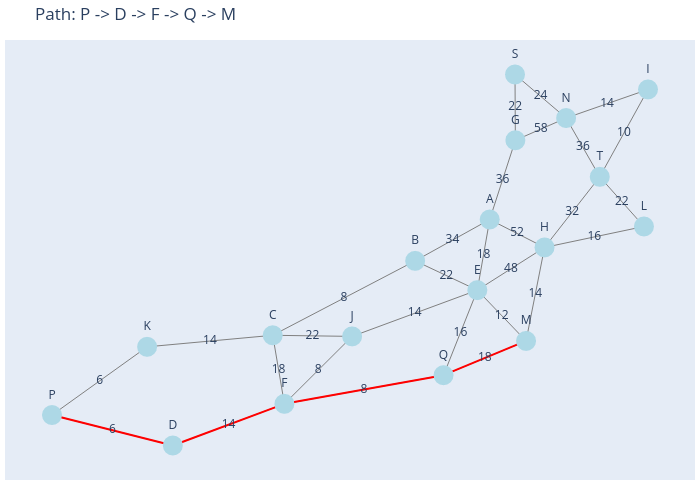
\includegraphics[width=0.7\linewidth]{Plots/P_D_F_Q_M.png}
    \caption{P-D-F-Q-M}
    \label{fig:enter-label}
\end{figure}
\begin{figure}
    \centering
    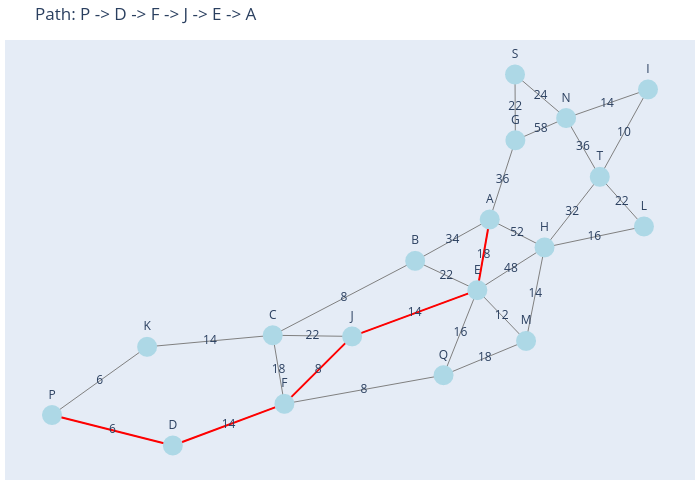
\includegraphics[width=0.7\linewidth]{Plots/P_D_F_J_E_A.png}
    \caption{P-D-F-J-E-A}
    \label{fig:enter-label}
\end{figure}
\begin{figure}
    \centering
    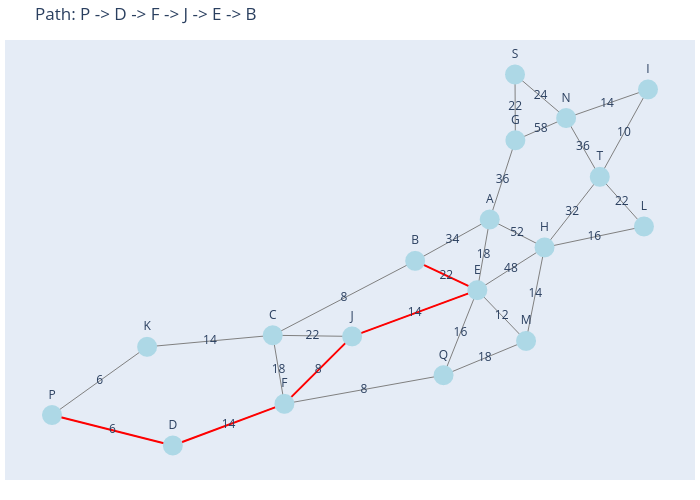
\includegraphics[width=0.7\linewidth]{Plots/P_D_F_J_E_B.png}
    \caption{P-D-F-J-E-B}
    \label{fig:enter-label}
\end{figure}
\begin{figure}
    \centering
    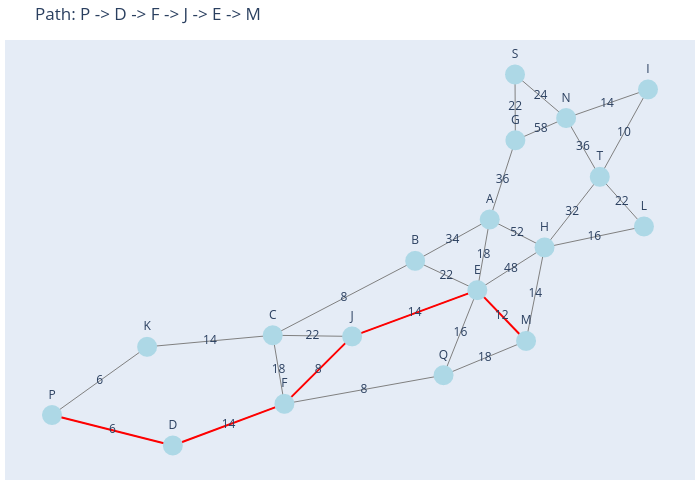
\includegraphics[width=0.7\linewidth]{Plots/P_D_F_J_E_M.png}
    \caption{P-D-F-J-E-M}
    \label{fig:enter-label}
\end{figure}
\begin{figure}
    \centering
    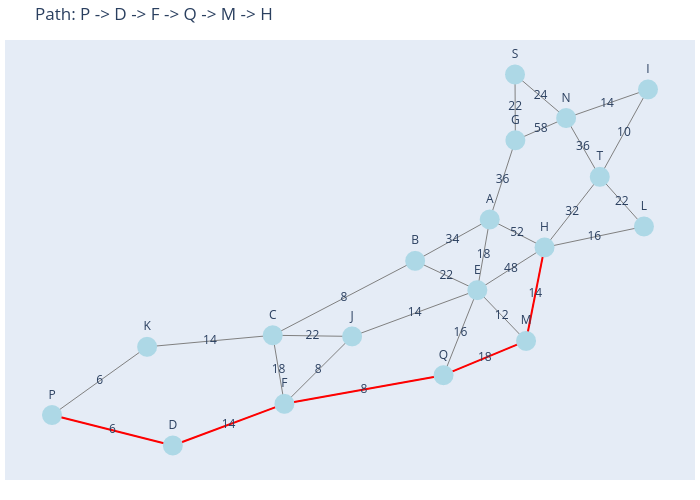
\includegraphics[width=0.7\linewidth]{Plots/P_D_F_Q_M_H.png}
    \caption{P-D-F-Q-M-H}
    \label{fig:enter-label}
\end{figure}
\begin{figure}
    \centering
    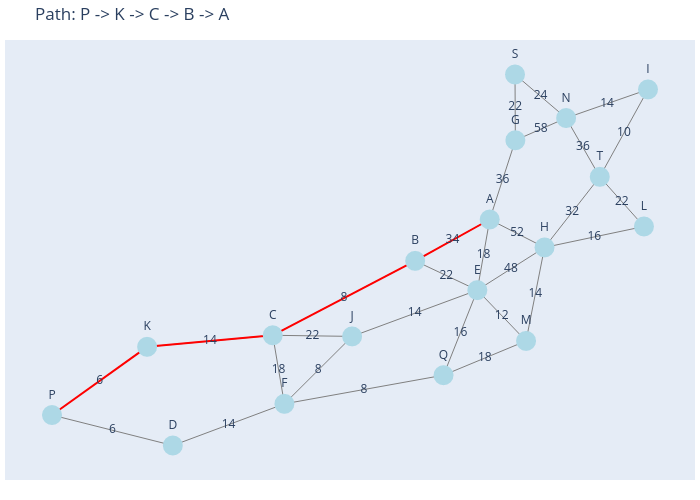
\includegraphics[width=0.7\linewidth]{Plots/P_K_C_B_A.png}
    \caption{P-K-C-B-A}
    \label{fig:enter-label}
\end{figure}
\begin{figure}
    \centering
    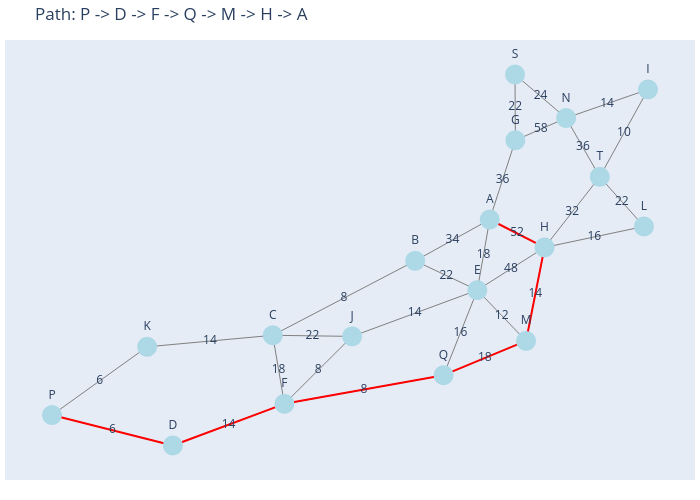
\includegraphics[width=0.7\linewidth]{Plots/P_D_F_Q_M_H_A.png}
    \caption{P-D-F-Q-M-H-A}
    \label{fig:enter-label}
\end{figure}
\begin{figure}
    \centering
    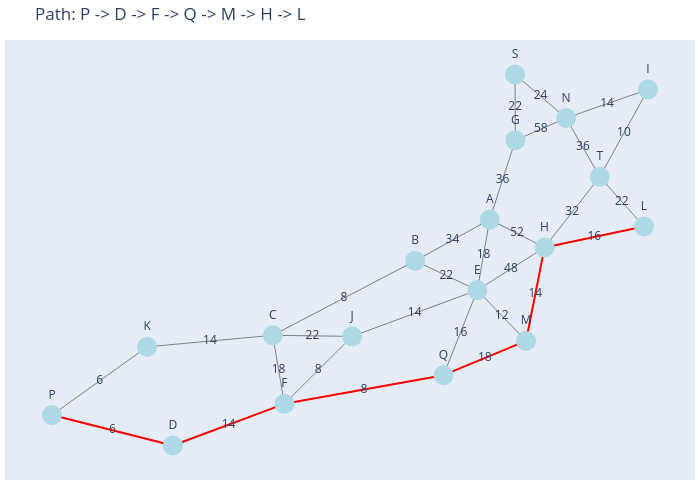
\includegraphics[width=0.7\linewidth]{Plots/P_D_F_Q_M_H_L.png}
    \caption{P-D-F-Q-M-H-L}
    \label{fig:enter-label}
\end{figure}
\begin{figure}
    \centering
    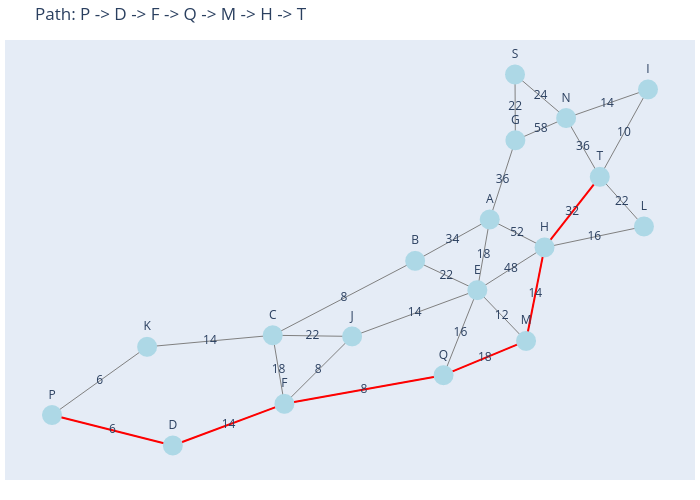
\includegraphics[width=0.7\linewidth]{Plots/P_D_F_Q_M_H_T.png}
    \caption{P-D-F-Q-M-H-T}
    \label{fig:enter-label}
\end{figure}
\begin{figure}
    \centering
    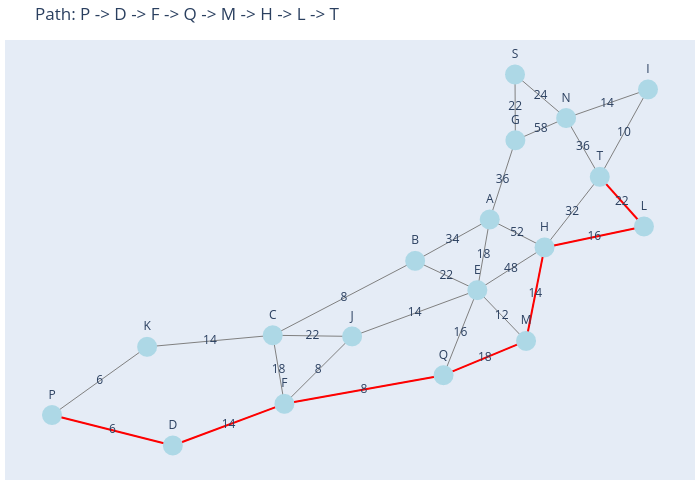
\includegraphics[width=0.7\linewidth]{Plots/P_D_F_Q_M_H_L_T.png}
    \caption{P-D-F-Q-M-H-L-T}
    \label{fig:enter-label}
\end{figure}
\begin{figure}
    \centering
    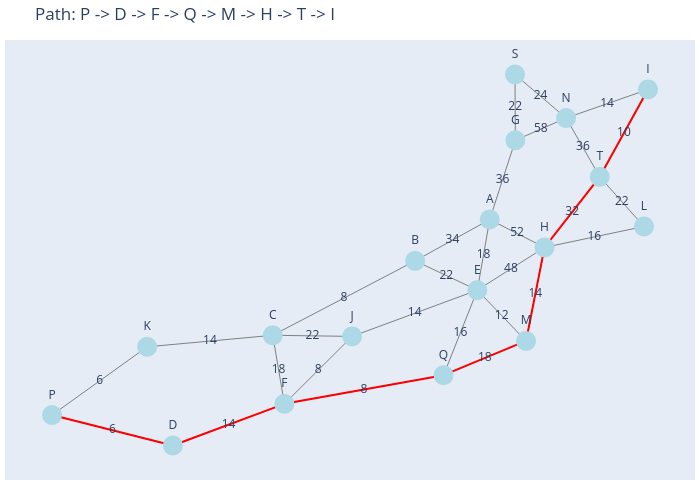
\includegraphics[width=0.7\linewidth]{Plots/P_D_F_Q_M_H_T_I.png}
    \caption{P-D-F-Q-M-H-T-I}
    \label{fig:enter-label}
\end{figure}
\begin{figure}
    \centering
    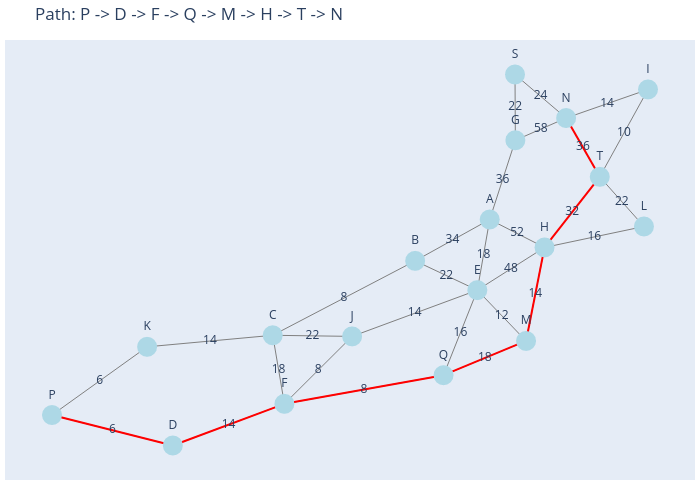
\includegraphics[width=0.7\linewidth]{Plots/P_D_F_Q_M_H_T_N.png}
    \caption{P-D-F-Q-M-H-T-N}
    \label{fig:enter-label}
\end{figure}
\begin{figure}
    \centering
    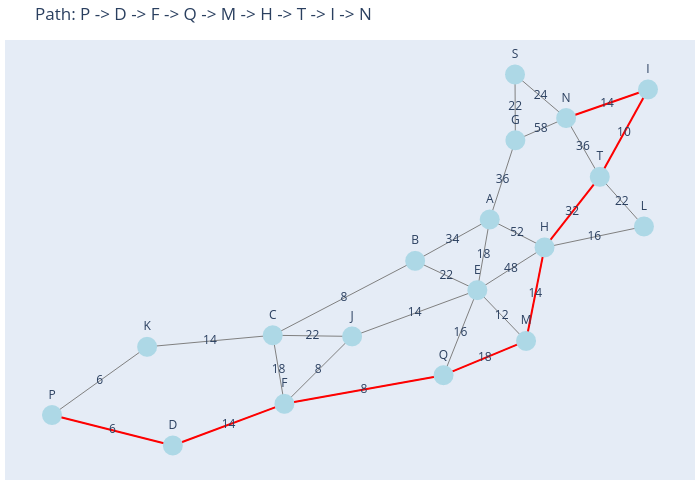
\includegraphics[width=0.7\linewidth]{Plots/P_D_F_Q_M_H_T_I_N.png}
    \caption{P-D-F-Q-M-H-T-I-N (Correct Answer)}
    \label{fig:enter-label}
\end{figure}
\begin{figure}
    \centering
    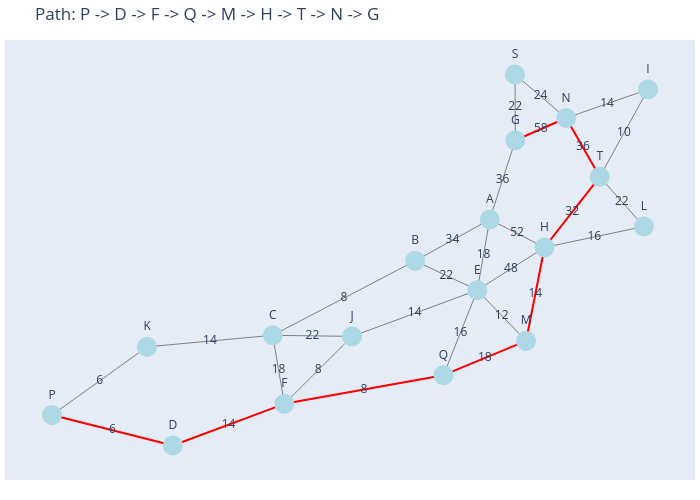
\includegraphics[width=0.7\linewidth]{Plots/P_D_F_Q_M_H_T_N_G.png}
    \caption{P-D-F-Q-M-H-T-N-G}
    \label{fig:enter-label}
\end{figure}
\begin{figure}
    \centering
    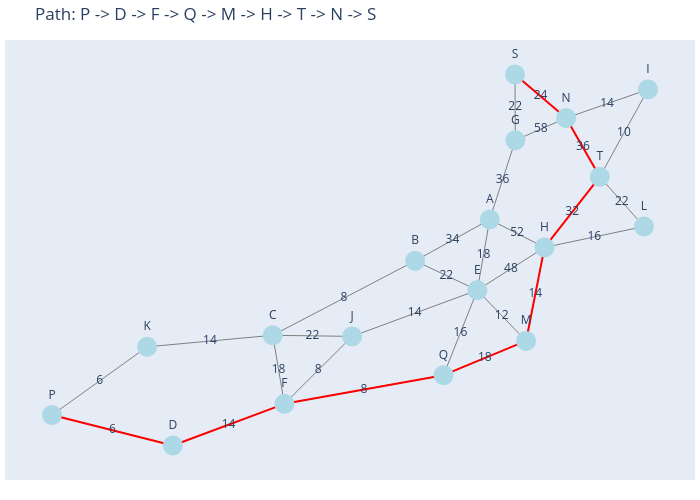
\includegraphics[width=0.7\linewidth]{Plots/P_D_F_Q_M_H_T_N_S.png}
    \caption{P-D-F-Q-M-H-T-N-S}
    \label{fig:enter-label}
\end{figure}

\chapter{Part 4}

\section{Kruskal Cabling Quote}
The school has asked Kruskal Cabling (Company C) to consider the issues and submit a proposal for construction. Kruskal Cabling has determined that the computer cable is to be laid in trenches which they dig rather than using the covered walkways at \$55 per meter. The trenches will use the shortest distance possible between buildings and the buildings will be connected via trenches to the computer network.
\includepdf[]{pdf/kruskal.pdf}

\section{Kruskal Cabling Construction Plan}
\begin{sidewaysfigure}[ht]
    \centering
    \includegraphics[width=1\linewidth]{img/Kruskal Cabling Plan.png}
    \caption{Kruskal Cabling Construction Plan.}
    \label{fig:enter-label}
\end{sidewaysfigure}

\section{Kruskal Cabling Trench Network}
\begin{sidewaysfigure}[ht]
    \centering
    \includegraphics[width=1\linewidth]{img/Trench Network.png}
    \caption{Kruskal Cabling Redrawn Trench Network.}
    \label{fig:enter-label}
\end{sidewaysfigure}

\section{Kruskal Cabling Trench Network Table}
\begin{table}[]
\begin{tabular}{lllll}
Start Node & End Node & Map Dist (mm) & Actual Dist (m) & Working Out \\
D & P & 3 & 6 & 2000÷1000 x 3 \\
P & K & 3 & 6 & 2000÷1000 x 3 \\
F & Q & 3 & 6 & 2000÷1000 x 3 \\
C & B & 4 & 8 & 2000÷1000 x 4 \\
F & J & 4 & 8 & 2000÷1000 x 4 \\
T & I & 4 & 8 & 2000÷1000 x 4 \\
D & F & 5 & 10 & 2000÷1000 x 5 \\
J & E & 5 & 10 & 2000÷1000 x 5 \\
M & H & 6 & 12 & 2000÷1000 x 6 \\
M & E & 6 & 12 & 2000÷1000 x 6 \\
K & C & 7 & 14 & 2000÷1000 x 7 \\
H & L & 7 & 14 & 2000÷1000 x 7 \\
L & T & 7 & 14 & 2000÷1000 x 7 \\
I & N & 7 & 14 & 2000÷1000 x 7 \\
E & A & 8 & 16 & 2000÷1000 x 8 \\
C & F & 9 & 18 & 2000÷1000 x 9 \\
C & J & 9 & 18 & 2000÷1000 x 9 \\
Q & M & 9 & 18 & 2000÷1000 x 9 \\
B & E & 10 & 20 & 2000÷1000 x 10 \\
A & G & 14 & 28 & 2000÷1000 x 14 \\
N & S & 11 & 22 & 2000÷1000 x 11 \\
B & A & 13 & 26 & 2000÷1000 x 13 \\
S & G & 10 & 20 & 2000÷1000 x 10 \\
H & E & 22 & 44 & 2000÷1000 x 22 \\
N & G & 28 & 56 & 2000÷1000 x 28 \\
 &  &  &  &  \\
 &  & Total Weight & 428 & 
\end{tabular}
\end{table}

\section{Kruskal Cabling Trench Network Table Working Out}
\begin{table}[]
\begin{tabular}{llllll}
Step & Start Node & End Node & Weight & Forms Cycle & Added \\
1 & D & P & 6 & FALSE & \cellcolor[HTML]{67FD9A}TRUE \\
2 & P & K & 6 & FALSE & \cellcolor[HTML]{67FD9A}TRUE \\
3 & F & Q & 6 & FALSE & \cellcolor[HTML]{67FD9A}TRUE \\
4 & C & B & 8 & FALSE & \cellcolor[HTML]{67FD9A}TRUE \\
5 & F & J & 8 & FALSE & \cellcolor[HTML]{67FD9A}TRUE \\
6 & T & I & 8 & FALSE & \cellcolor[HTML]{67FD9A}TRUE \\
7 & D & F & 10 & FALSE & \cellcolor[HTML]{67FD9A}TRUE \\
8 & J & E & 10 & FALSE & \cellcolor[HTML]{67FD9A}TRUE \\
9 & M & H & 12 & FALSE & \cellcolor[HTML]{67FD9A}TRUE \\
10 & M & E & 12 & FALSE & \cellcolor[HTML]{67FD9A}TRUE \\
11 & K & C & 14 & FALSE & \cellcolor[HTML]{67FD9A}TRUE \\
12 & H & L & 14 & FALSE & \cellcolor[HTML]{67FD9A}TRUE \\
13 & L & T & 14 & FALSE & \cellcolor[HTML]{67FD9A}TRUE \\
14 & I & N & 14 & FALSE & \cellcolor[HTML]{67FD9A}TRUE \\
15 & E & A & 16 & FALSE & \cellcolor[HTML]{67FD9A}TRUE \\
16 & C & F & 18 & TRUE & \cellcolor[HTML]{FD6864}FALSE \\
17 & C & J & 18 & TRUE & \cellcolor[HTML]{FD6864}FALSE \\
18 & Q & M & 18 & TRUE & \cellcolor[HTML]{FD6864}FALSE \\
19 & B & E & 20 & TRUE & \cellcolor[HTML]{FD6864}FALSE \\
20 & S & G & 20 & FALSE & \cellcolor[HTML]{67FD9A}TRUE \\
21 & N & S & 22 & FALSE & \cellcolor[HTML]{67FD9A}TRUE \\
22 & B & A & 26 & TRUE & \cellcolor[HTML]{FD6864}FALSE \\
23 & A & G & 28 & TRUE & \cellcolor[HTML]{FD6864}FALSE \\
24 & H & E & 44 & TRUE & \cellcolor[HTML]{FD6864}FALSE \\
25 & N & G & 55 & TRUE & \cellcolor[HTML]{FD6864}FALSE \\
 &  &  &  &  &  \\
 &  & Total Weight & 190 &  &  \\
 &  & Total Cost & \$10,450.00 &  & 
\end{tabular}
\caption{}
\label{tab:my-table}
\end{table}

\begin{sidewaysfigure}
    \centering
    \includegraphics[width=1\linewidth]{Trenches/1.png}
    \caption{D-P}
    \label{fig:enter-label}
\end{sidewaysfigure}
\begin{sidewaysfigure}
    \centering
    \includegraphics[width=1\linewidth]{Trenches/2.png}
    \caption{P-K}
    \label{fig:enter-label}
\end{sidewaysfigure}
\begin{sidewaysfigure}
    \centering
    \includegraphics[width=1\linewidth]{Trenches/3.png}
    \caption{F-Q}
    \label{fig:enter-label}
\end{sidewaysfigure}
\begin{sidewaysfigure}
    \centering
    \includegraphics[width=1\linewidth]{Trenches/4.png}
    \caption{C-B}
    \label{fig:enter-label}
\end{sidewaysfigure}
\begin{sidewaysfigure}
    \centering
    \includegraphics[width=1\linewidth]{Trenches/5.png}
    \caption{F-J}
    \label{fig:enter-label}
\end{sidewaysfigure}
\begin{sidewaysfigure}
    \centering
    \includegraphics[width=1\linewidth]{Trenches/6.png}
    \caption{T-I}
    \label{fig:enter-label}
\end{sidewaysfigure}
\begin{sidewaysfigure}
    \centering
    \includegraphics[width=1\linewidth]{Trenches/7.png}
    \caption{D-F}
    \label{fig:enter-label}
\end{sidewaysfigure}
\begin{sidewaysfigure}
    \centering
    \includegraphics[width=1\linewidth]{Trenches/8.png}
    \caption{J-E}
    \label{fig:enter-label}
\end{sidewaysfigure}
\begin{sidewaysfigure}
    \centering
    \includegraphics[width=1\linewidth]{Trenches/9.png}
    \caption{M-H}
    \label{fig:enter-label}
\end{sidewaysfigure}
\begin{sidewaysfigure}
    \centering
    \includegraphics[width=1\linewidth]{Trenches/10.png}
    \caption{M-E}
    \label{fig:enter-label}
\end{sidewaysfigure}
\begin{sidewaysfigure}
    \centering
    \includegraphics[width=1\linewidth]{Trenches/12.png}
    \caption{H-L}
    \label{fig:enter-label}
\end{sidewaysfigure}
\begin{sidewaysfigure}
    \centering
    \includegraphics[width=1\linewidth]{Trenches/13.png}
    \caption{L-T}
    \label{fig:enter-label}
\end{sidewaysfigure}
\begin{sidewaysfigure}
    \centering
    \includegraphics[width=1\linewidth]{Trenches/14.png}
    \caption{I-N}
    \label{fig:enter-label}
\end{sidewaysfigure}
\begin{sidewaysfigure}
    \centering
    \includegraphics[width=1\linewidth]{Trenches/15.png}
    \caption{E-A}
    \label{fig:enter-label}
\end{sidewaysfigure}
\begin{sidewaysfigure}
    \centering
    \includegraphics[width=1\linewidth]{Trenches/16.png}
    \caption{A-G}
    \label{fig:enter-label}
\end{sidewaysfigure}
\begin{sidewaysfigure}
    \centering
    \includegraphics[width=1\linewidth]{Trenches/17.png}
    \caption{N-S}
    \label{fig:enter-label}
\end{sidewaysfigure}

\chapter{Part 5}
\section{PidgeonHole Expert Sparky's Quote}
As a forth and final proposal, the school approaches PidgeonHole Expert Sparky's (Company D), PidgeonHole decides it will use a combination of trenches and covered walkways. Their aim to connect every building using the shortest distance possible. The covered walkway cable will cost them \$45 per meter, and the trenches will remain at \$55 per meter.

\includepdf[]{pdf/pidgeonhole.pdf}

\section{PidgeonHole Expert Sparky's Construction Plan}
\begin{sidewaysfigure}[ht]
    \centering
    \includegraphics[width=1\linewidth]{img/PidgeonHole Construction Plan.png}
    \caption{PidgeonHole Construction Plan.}
    \label{fig:enter-label}
\end{sidewaysfigure}

\section{PidgeonHole Expert Sparky's Table 1}
\begin{table}[]
\begin{tabular}{llll}
Start Node & End Node & Weight & Is Trench \\
\rowcolor[HTML]{FFCCC9} 
D & P & 6 & TRUE \\
\rowcolor[HTML]{FFCCC9} 
P & K & 6 & TRUE \\
F & Q & 6 & TRUE \\
\rowcolor[HTML]{FFCCC9} 
C & B & 8 & TRUE \\
\rowcolor[HTML]{FFCCC9} 
F & J & 8 & TRUE \\
T & I & 8 & TRUE \\
J & E & 12 & TRUE \\
M & H & 12 & TRUE \\
\rowcolor[HTML]{FFCCC9} 
M & E & 12 & TRUE \\
\rowcolor[HTML]{FFCCC9} 
K & C & 14 & TRUE \\
H & L & 14 & TRUE \\
L & T & 14 & TRUE \\
\rowcolor[HTML]{FFCCC9} 
I & N & 14 & TRUE \\
E & A & 16 & TRUE \\
G & S & 20 & TRUE \\
N & S & 22 & TRUE \\
\rowcolor[HTML]{9AFF99} 
P & D & 6 & FALSE \\
\rowcolor[HTML]{9AFF99} 
P & K & 6 & FALSE \\
\rowcolor[HTML]{9AFF99} 
K & C & 14 & FALSE \\
D & F & 14 & FALSE \\
F & C & 18 & FALSE \\
\rowcolor[HTML]{67FD9A} 
F & J & 8 & FALSE \\
F & Q & 8 & FALSE \\
\rowcolor[HTML]{9AFF99} 
C & B & 8 & FALSE \\
C & J & 22 & FALSE \\
C & F & 18 & FALSE \\
B & A & 34 & FALSE \\
B & E & 22 & FALSE \\
J & E & 14 & FALSE \\
Q & E & 16 & FALSE \\
Q & M & 18 & FALSE \\
A & G & 36 & FALSE \\
A & H & 52 & FALSE \\
E & J & 14 & FALSE \\
E & A & 18 & FALSE \\
E & H & 48 & FALSE \\
\rowcolor[HTML]{9AFF99} 
E & M & 12 & FALSE \\
M & H & 14 & FALSE \\
H & T & 32 & FALSE \\
H & L & 16 & FALSE \\
L & T & 22 & FALSE \\
T & N & 36 & FALSE \\
T & I & 10 & FALSE \\
\rowcolor[HTML]{9AFF99} 
I & N & 14 & FALSE \\
N & G & 58 & FALSE \\
N & S & 24 & FALSE \\
S & G & 22 & FALSE
\end{tabular}
\caption{If Trench Weight is = to Walkway Weight = Removal}
\label{tab:my-table}
\end{table}

\begin{sidewaysfigure}[ht]
    \centering
    \includegraphics[width=1\linewidth]{img/PigeonHole NW1.png}
    \caption{PidgeonHole Network 1. Data on Table 6.1}
    \label{fig:enter-label}
\end{sidewaysfigure}

\section{PidgeonHole Expert Sparky's Table 2}
\begin{table}[]
\begin{tabular}{lllll}
Start Node & End Node & Weight & Is Trench & Trench is -4m \\
\rowcolor[HTML]{FFCCC9} 
F & Q & 6 & TRUE & 0 \\
\rowcolor[HTML]{FFCCC9} 
T & I & 8 & TRUE & 0 \\
\rowcolor[HTML]{FFCCC9} 
J & E & 12 & TRUE & 0 \\
\rowcolor[HTML]{FFCCC9} 
M & H & 12 & TRUE & 0 \\
\rowcolor[HTML]{FFCCC9} 
H & L & 14 & TRUE & 0 \\
L & T & 14 & TRUE & 1 \\
\rowcolor[HTML]{FFCCC9} 
E & A & 16 & TRUE & 0 \\
\rowcolor[HTML]{FFCCC9} 
G & S & 20 & TRUE & 0 \\
\rowcolor[HTML]{FFCCC9} 
N & S & 22 & TRUE & 0 \\
P & D & 6 & FALSE & - \\
P & K & 6 & FALSE & - \\
K & C & 14 & FALSE & - \\
D & F & 14 & FALSE & - \\
F & C & 18 & FALSE & - \\
F & J & 8 & FALSE & - \\
\rowcolor[HTML]{9AFF99} 
F & Q & 8 & FALSE & - \\
C & B & 8 & FALSE & - \\
C & J & 22 & FALSE & - \\
C & F & 18 & FALSE & - \\
B & A & 34 & FALSE & - \\
B & E & 22 & FALSE & - \\
J & E & 14 & FALSE & - \\
Q & E & 16 & FALSE & - \\
Q & M & 18 & FALSE & - \\
A & G & 36 & FALSE & - \\
A & H & 52 & FALSE & - \\
\rowcolor[HTML]{9AFF99} 
E & J & 14 & FALSE & - \\
\rowcolor[HTML]{9AFF99} 
E & A & 18 & FALSE & - \\
E & H & 48 & FALSE & - \\
E & M & 12 & FALSE & - \\
\rowcolor[HTML]{9AFF99} 
M & H & 14 & FALSE & - \\
H & T & 32 & FALSE & - \\
\rowcolor[HTML]{9AFF99} 
H & L & 16 & FALSE & - \\
\rowcolor[HTML]{FFCCC9} 
L & T & 22 & FALSE & - \\
T & N & 36 & FALSE & - \\
\rowcolor[HTML]{9AFF99} 
T & I & 10 & FALSE & - \\
I & N & 14 & FALSE & - \\
N & G & 58 & FALSE & - \\
\rowcolor[HTML]{9AFF99} 
N & S & 24 & FALSE & - \\
\rowcolor[HTML]{9AFF99} 
S & G & 22 & FALSE & -
\end{tabular}
\caption{If Trench Weight is not less that 4 of Walkway Weight = Removal}
\label{tab:my-table}
\end{table}

\begin{sidewaysfigure}[ht]
    \centering
    \includegraphics[width=1\linewidth]{img/PigeonHole NW2.png}
    \caption{PidgeonHole Network 2. Data on Table 6.2}
    \label{fig:enter-label}
\end{sidewaysfigure}

\section{PidgeonHole Expert Sparky's Final Network Table 3}
\begin{table}[]
\begin{tabular}{llll}
Start Node & End Node & Weight & Is Trench \\
L & T & 14 & TRUE \\
P & D & 6 & FALSE \\
P & K & 6 & FALSE \\
K & C & 14 & FALSE \\
D & F & 14 & FALSE \\
F & C & 18 & FALSE \\
F & J & 8 & FALSE \\
F & Q & 8 & FALSE \\
C & B & 8 & FALSE \\
C & J & 22 & FALSE \\
C & F & 18 & FALSE \\
B & A & 34 & FALSE \\
B & E & 22 & FALSE \\
J & E & 14 & FALSE \\
Q & E & 16 & FALSE \\
Q & M & 18 & FALSE \\
A & G & 36 & FALSE \\
A & H & 52 & FALSE \\
E & J & 14 & FALSE \\
E & A & 18 & FALSE \\
E & H & 48 & FALSE \\
E & M & 12 & FALSE \\
M & H & 14 & FALSE \\
H & T & 32 & FALSE \\
H & L & 16 & FALSE \\
T & N & 36 & FALSE \\
T & I & 10 & FALSE \\
I & N & 14 & FALSE \\
N & G & 58 & FALSE \\
N & S & 24 & FALSE \\
S & G & 22 & FALSE
\end{tabular}
\caption{Final Network Table}
\label{tab:my-table}
\end{table}

\begin{sidewaysfigure}[ht]
    \centering
    \includegraphics[width=1\linewidth]{img/PigeonHole NW3.png}
    \caption{PidgeonHole Network 3. Data on Table 6.3}
    \label{fig:enter-label}
\end{sidewaysfigure}

\section{PidgeonHole Expert Sparky's Working Out}
\begin{table}[]
\begin{tabular}{llllllll}
Step & Start Node & End Node & Weight & Is Trench & Forms Cycle & Is Lowest Edge & Added \\
0 & D & P & 6 & FALSE & FALSE & TRUE & \cellcolor[HTML]{9AFF99}TRUE \\
1 & P & K & 6 & FALSE & FALSE & TRUE & \cellcolor[HTML]{9AFF99}TRUE \\
2 & K & C & 14 & FALSE & FALSE & TRUE & \cellcolor[HTML]{9AFF99}TRUE \\
3 & C & B & 8 & FALSE & FALSE & TRUE & \cellcolor[HTML]{9AFF99}TRUE \\
4 & E & B & 22 & FALSE & FALSE & FALSE & \cellcolor[HTML]{FFCCC9}FALSE \\
5 & D & F & 14 & FALSE & FALSE & TRUE & \cellcolor[HTML]{9AFF99}TRUE \\
6 & F & J & 8 & FALSE & FALSE & TRUE & \cellcolor[HTML]{9AFF99}TRUE \\
7 & J & E & 14 & FALSE & FALSE & TRUE & \cellcolor[HTML]{9AFF99}TRUE \\
8 & E & M & 12 & FALSE & FALSE & TRUE & \cellcolor[HTML]{9AFF99}TRUE \\
9 & M & H & 14 & FALSE & FALSE & TRUE & \cellcolor[HTML]{9AFF99}TRUE \\
10 & H & L & 16 & FALSE & FALSE & TRUE & \cellcolor[HTML]{9AFF99}TRUE \\
11 & L & T & 14 & \cellcolor[HTML]{9AFF99}TRUE & FALSE & TRUE & \cellcolor[HTML]{9AFF99}TRUE \\
12 & T & I & 10 & FALSE & FALSE & TRUE & \cellcolor[HTML]{9AFF99}TRUE \\
13 & I & N & 14 & FALSE & FALSE & TRUE & \cellcolor[HTML]{9AFF99}TRUE \\
14 & N & S & 24 & FALSE & FALSE & TRUE & \cellcolor[HTML]{9AFF99}TRUE \\
15 & G & S & 22 & FALSE & FALSE & FALSE & \cellcolor[HTML]{9AFF99}TRUE \\
16 & E & A & 18 & FALSE & FALSE & FALSE & \cellcolor[HTML]{FFCCC9}FALSE \\
17 & F & Q & 8 & FALSE & FALSE & TRUE & \cellcolor[HTML]{9AFF99}TRUE \\
18 & Q & E & 16 & FALSE & FALSE & FALSE & \cellcolor[HTML]{FFCCC9}FALSE \\
19 & M & Q & 18 & FALSE & TRUE & FALSE & \cellcolor[HTML]{FFCCC9}FALSE \\
20 & F & C & 18 & FALSE & TRUE & FALSE & \cellcolor[HTML]{FFCCC9}FALSE \\
21 & Q & M & 18 & FALSE & TRUE & FALSE & \cellcolor[HTML]{FFCCC9}FALSE \\
22 & J & C & 22 & FALSE & TRUE & FALSE & \cellcolor[HTML]{FFCCC9}FALSE \\
23 & T & H & 32 & FALSE & TRUE & FALSE & \cellcolor[HTML]{FFCCC9}FALSE \\
24 & A & B & 34 & FALSE & TRUE & FALSE & \cellcolor[HTML]{FFCCC9}FALSE \\
25 & T & N & 36 & FALSE & TRUE & FALSE & \cellcolor[HTML]{FFCCC9}FALSE \\
26 & A & G & 36 & FALSE & TRUE & FALSE & \cellcolor[HTML]{FFCCC9}FALSE \\
27 & H & E & 48 & FALSE & TRUE & FALSE & \cellcolor[HTML]{FFCCC9}FALSE \\
28 & H & A & 52 & FALSE & TRUE & FALSE & \cellcolor[HTML]{FFCCC9}FALSE \\
29 & N & G & 58 & FALSE & TRUE & FALSE & \cellcolor[HTML]{FFCCC9}FALSE \\
 &  &  &  &  &  &  &  \\
 & Total Trench Weight &  & 14 &  &  &  &  \\
 & Total Path Weight &  & 200 &  &  &  &  \\
 &  &  &  &  &  &  &  \\
 & Total Trench Cost &  & 770 &  &  &  &  \\
 & Total Path Cost &  & 9000 &  &  &  &  \\
 &  &  &  &  &  &  &  \\
 & \cellcolor[HTML]{9AFF99}Total Cost & \cellcolor[HTML]{9AFF99} & \cellcolor[HTML]{9AFF99}\$9,770.00 &  &  &  & 
\end{tabular}
\caption{Network Table, Prim's Algorithm Calculation}
\label{tab:my-table}
\end{table}

\begin{sidewaysfigure}
    \centering
    \includegraphics[width=1\linewidth]{q5_plots/1.png}
    \caption{D-P}
    \label{fig:enter-label}
\end{sidewaysfigure}
\begin{sidewaysfigure}
    \centering
    \includegraphics[width=1\linewidth]{q5_plots/2.png}
    \caption{P-K}
    \label{fig:enter-label}
\end{sidewaysfigure}
\begin{sidewaysfigure}
    \centering
    \includegraphics[width=1\linewidth]{q5_plots/3.png}
    \caption{K-C}
    \label{fig:enter-label}
\end{sidewaysfigure}
\begin{sidewaysfigure}
    \centering
    \includegraphics[width=1\linewidth]{q5_plots/4.png}
    \caption{C-B}
    \label{fig:enter-label}
\end{sidewaysfigure}
\begin{sidewaysfigure}
    \centering
    \includegraphics[width=1\linewidth]{q5_plots/5.png}
    \caption{D-F}
    \label{fig:enter-label}
\end{sidewaysfigure}
\begin{sidewaysfigure}
    \centering
    \includegraphics[width=1\linewidth]{q5_plots/6.png}
    \caption{F-J}
    \label{fig:enter-label}
\end{sidewaysfigure}
\begin{sidewaysfigure}
    \centering
    \includegraphics[width=1\linewidth]{q5_plots/7.png}
    \caption{J-E}
    \label{fig:enter-label}
\end{sidewaysfigure}
\begin{sidewaysfigure}
    \centering
    \includegraphics[width=1\linewidth]{q5_plots/8.png}
    \caption{E-M}
    \label{fig:enter-label}
\end{sidewaysfigure}
\begin{sidewaysfigure}
    \centering
    \includegraphics[width=1\linewidth]{q5_plots/9.png}
    \caption{M-H}
    \label{fig:enter-label}
\end{sidewaysfigure}
\begin{sidewaysfigure}
    \centering
    \includegraphics[width=1\linewidth]{q5_plots/10.png}
    \caption{H-L}
    \label{fig:enter-label}
\end{sidewaysfigure}
\begin{sidewaysfigure}
    \centering
    \includegraphics[width=1\linewidth]{q5_plots/11.png}
    \caption{L-T}
    \label{fig:enter-label}
\end{sidewaysfigure}
\begin{sidewaysfigure}
    \centering
    \includegraphics[width=1\linewidth]{q5_plots/12.png}
    \caption{T-I}
    \label{fig:enter-label}
\end{sidewaysfigure}
\begin{sidewaysfigure}
    \centering
    \includegraphics[width=1\linewidth]{q5_plots/13.png}
    \caption{I-N}
    \label{fig:enter-label}
\end{sidewaysfigure}
\begin{sidewaysfigure}
    \centering
    \includegraphics[width=1\linewidth]{q5_plots/14.png}
    \caption{N-S}
    \label{fig:enter-label}
\end{sidewaysfigure}
\begin{sidewaysfigure}
    \centering
    \includegraphics[width=1\linewidth]{q5_plots/15.png}
    \caption{S-G}
    \label{fig:enter-label}
\end{sidewaysfigure}
\begin{sidewaysfigure}
    \centering
    \includegraphics[width=1\linewidth]{q5_plots/16.png}
    \caption{F-Q (Final Network MST)}
    \label{fig:enter-label}
\end{sidewaysfigure}

\chapter{Part 6}
\section{Company Proposal Comparison}

The NSW Department of Education has received quotes from 4 companies to re-cable the network cables at Math More High School, Math More High School is currently comprised of 29 existing walkways (edges) where the cables can be put, and 18 buildings (nodes or vertices). Each meter of walkway cable will cost \$45, while trench cabling will cost \$55.
The four contacted companies have been Al-Khwaizmi Simple Data (Company A), Dijkstra Data (Company B), Kruskal Cabling (Company C), and PidgeonHole Expert Sparky's (Company D).
The executive for Math More High School has tasked each company with its own construction plan.
Al-Khwaizmi Simple Data must create a minimum spanning tree of the network using the existing walkways.
Dijkstra Data must create a shortest path from building P (Workshop) and building N (English), only connecting the buildings on said shortest path.
Kruskal Cabling has been tasked with making new trenches to place the cables in and create a new minimum spanning tree using the trench paths.
PidgeonHole Expert Sparky's has been tasked with creating a minimum spanning tree combining both trenches and the pre-existing walkways.

\section{Al-Khwaizmi Simple Data Proposition}
Dear Customer,
With your requests of using the pre existing walkways for the cables we can quote you that each meter will cost \$45, additionally using a minimum spanning tree, we can get you the lowest cost of cable due to us using the path with the least weight, this is achieved by using Prim's Algorithm, in this algorithm it can find the minimum spanning tree by picking a node and selecting
the edge with the lowest weight, excluding edges that form a cycle or that are not the lowest edge connected to a node, this is repeated until there is a minimum spanning tree of nodes and edges.
If you have any questions please look at the construction plan attached to this document and the calculation below. If you are not satisfied please give us a call so we can give you a quote to your liking. \\

Meters of Cable: 238m \\
Cost of Cables (including GST): \textbf{\$11,781.00} \\

\section{Dijkstra Data Proposition}
Dear NSW DoE,
You have requested to us to only connect the building between P and N that have the shortest path. For this we have used our own in house developed algorithm called Dijkstra's Algorithm, this algorithm calculates the shortest distance from one node (vertex) to another node, this is done by first choosing the starting node, then it checks which nodes are known (connected) to it and the distance (weight), if unknown the distance if set as 'inf', then the total distance is calculating by adding the edges connecting the start node to end node, this is repeated until the final desired node (vertex) is reached.
If any questions may arise
please don't hesitate to contact us so we can give you the best experience. \\

Meters of Cable: 122m \\
Cost of Cables (including GST): \textbf{\$6,039.00} \\

\section{Kruskal Cabling Proposition}
Dear Customer,
Thank you for providing your building schematics as this has enables us to find the optimal cost per meter ratio. We have used this to create a plan for the data cables to go into 4m deep trenches below ground. Our site planners and engineers have used a new network algorithm called Kruskal's Algorithm developed in house by us. 
Firstly we drew new edges for each of the nodes and
then we made new edge conntections (trenches) to the neighbouring nodes (verticies), then we used Kruskal's Algorithm to create a minimum spanning tree (MST) of a network by sorting all edges by their distance (weight), then its checked if adding the edge would form a cycle, if it does form a cycle the edge is not added to the MST, if it does not form a cycle it is added to the MST.
this algorithm is useful as to provide the minimal amount of weight needed in a network.
The following construction plan is located in this document below, feel free to check them out and report us if you notice anything that needs changing or fixing. \\

Meters of Trench Cable: 190m \\
Cost of Cables (including GST): \textbf{\$11,495.00} \\

\section{PidgeonHole Expert Sparky's Proposition}
Dear Client,
We are pleased to do all your sparky and data needs at PidgeonHole Expert Sparky's. We have used your existing building plans, after evaluating it we see that a combination of using the existing walkways and new trenches would be the most cost effective plan. 
Using the said plan we drew new edges for the trenches from one node (vertex) to other neighbouring nodes (vertices), in addition to this we also added the pre-existing walkway paths, using this we implemented Prims algorithm, a algorithm that builds a minimum spanning tree from one node to other nodes using the shortest edge, however we have implemented some changes, for the walkways if the cable distance was more than 4m+ of the
trenches, the trenchers were preferred, so there is a 4m+/- for the walkways for the most cost effective plan. The following new
building schematic can be found in this document, shall any problems arise please contact us asap. Thank you for being a
customer of PidgeonHole Expert Sparky's, we hope to see you soon. \\

Meters of Walkway Cable: 200m \\
Meters of Trench Cable:	14m \\
\\
Cost of Walkway Cable: \$9,000.00 \\
Cost of Trench Cable: \$770.00\\
\\
Total Cost (including GST): \textbf{\$10,747.00} \\

\newpage
\section{Comparison of Company Costs}

\begin{table}[]
\begin{tabular}{lllll}
 & Al-Khwaizmi & Dijkstra & Kruskal & PidgeonHole \\
 & \$11,781.00 & \$6,039.00 & \$11,495.00 & \$10,747.00 \\
Al-Khwaizmi & - & \cellcolor[HTML]{9AFF99}-64.44\% & \cellcolor[HTML]{9AFF99}-2.46\% & \cellcolor[HTML]{9AFF99}-9.18\% \\
Dijkstra & \cellcolor[HTML]{FFCCC9}64.44\% & - & \cellcolor[HTML]{FFCCC9}62.23\% & \cellcolor[HTML]{FFCCC9}56.09\% \\
Kruskal & \cellcolor[HTML]{FFCCC9}2.46\% & \cellcolor[HTML]{9AFF99}-62.23\% & - & \cellcolor[HTML]{9AFF99}-6.73\% \\
PidgeonHole & \cellcolor[HTML]{FFCCC9}9.18\% & \cellcolor[HTML]{9AFF99}-56.09\% & \cellcolor[HTML]{FFCCC9}6.73\% & -
\end{tabular}
\caption{Cost Comparison Table}
\label{tab:my-table}
\end{table}

\begin{table}[]
    \resizebox{\textwidth}{!}{%
    \begin{tabular}{lllll}
     & Al-Khwaizmi & Dijkstra & Kruskal & PidgeonHole \\
     & \$11,781.00 & \$6,039.00 & \$11,495.00 & \$10,747.00 \\
    Al-Khwaizmi & - & \cellcolor[HTML]{9AFF99}(6039 - 11781 ) \textbackslash{}÷ ((11781 + 11781) \textbackslash{}÷ ) & \cellcolor[HTML]{9AFF99}(11495 - 11781) \textbackslash{}÷ ((11495 + 11781) \textbackslash{}÷ 2 ) & \cellcolor[HTML]{9AFF99}(10747 - 11781) \textbackslash{}÷ ((10747 + 11781) \textbackslash{}÷ 2 ) \\
    Dijkstra & \cellcolor[HTML]{FFCCC9}(11781 - 6039 ) \textbackslash{}÷ ((11781 + 6039) \textbackslash{}÷ 2 ) & - & \cellcolor[HTML]{FFCCC9}(11495 - 6039) \textbackslash{}÷ ((11495 + 6039) \textbackslash{}÷ 2 ) & \cellcolor[HTML]{FFCCC9}(10747 - 6039) \textbackslash{}÷ ((10747 + 6039) \textbackslash{}÷ 2 ) \\
    Kruskal & \cellcolor[HTML]{FFCCC9}(11781 - 11495 ) \textbackslash{}÷ ((11781 + 11495) \textbackslash{}÷ 2 ) & \cellcolor[HTML]{9AFF99}(6039 - 11495 ) \textbackslash{}÷ ((11781 + 11495) \textbackslash{}÷ 2 ) & - & \cellcolor[HTML]{9AFF99}(10747 - 11495) \textbackslash{}÷ ((10747 + 11495) \textbackslash{}÷ 2 ) \\
    PidgeonHole & \cellcolor[HTML]{FFCCC9}(11781 - 10747 ) \textbackslash{}÷ ((11781 + 10747) \textbackslash{}÷ 2 ) & \cellcolor[HTML]{9AFF99}(6039 - 10747 ) \textbackslash{}÷ ((11781 + 10747) \textbackslash{}÷ 2 ) & \cellcolor[HTML]{FFCCC9}(11495 - 10747) \textbackslash{}÷ ((11495 + 10747) \textbackslash{}÷ 2 ) & -
    \end{tabular}%
    }
    \caption{Cost Comparison Table Working Out}
    \label{tab:my-table}
    \end{table}

The Formula for comparing the cost used is
\begin{equation}
    \frac{[V_{1}-V_{2}]}{\frac{(V_{1}+V_{2})}{2}}

    V_{1} = Cost 1 \\
    V_{2} = Cost 2 \\
\end{equation}

As seen above in Table 7.1 The largest amount of reduction in cost is Dijkstra Data at -64.44\%, but this is not the best option due to it only connecting the buildings between P-N this means buildings K, J, C, E, B, A, L, G, and S, are not connected. \\
The best choice is for this would be PidgeonHole Expert Sparky's as they would connect all buildings at a savings of 9.18\% when compared to Al-Khwaizmi Simple Data, and 6.73\% savings when compared to Kruskal Cabling. \\


\begin{table}[]
\resizebox{\textwidth}{!}{%
\begin{tabular}{lllll}
 & Al-Khawaimi & Dijkstra & Kruskal & Pidgeon \\
\cellcolor[HTML]{9AFF99}Advantages & \begin{tabular}[c]{@{}l@{}}Connects All Buildings\\ Walkway Cabling can easily be replaced if not working\\ Time Effective, Less time required when comparing to trenches\end{tabular} & \begin{tabular}[c]{@{}l@{}}Cheap\\ Time Effective\\ Walkway Cabling can easily be replaced if not working\end{tabular} & \begin{tabular}[c]{@{}l@{}}Connects All Buildings\\ Trenches keep cables underground and protected\end{tabular} & \begin{tabular}[c]{@{}l@{}}Connects All Buildings\\ Hybrid of Trenches and Walkway cables keeps it effective\\ Only requires one trench\\ Walkway Cabling can easily be replaced if not working\end{tabular} \\
\cellcolor[HTML]{FFCCC9}Disadvantages & \begin{tabular}[c]{@{}l@{}}Expensive\\ Some walkways are not effective, shorter path possible\end{tabular} & Only Connects Buildings on P-NSome buildings wont get networking & \begin{tabular}[c]{@{}l@{}}Trenches need additional safety precautions\\ Trenches will take longer to dig and run cables\end{tabular} & \begin{tabular}[c]{@{}l@{}}Trenches need additional safety precautions\\ Trenches will take longer to dig and run cables\end{tabular}
\end{tabular}%
}
\caption{Advantages And Disadvantages Of Companies}
\label{tab:my-table}
\end{table}

\section{Final Choice}

The \textbf{best choice} for networking Math More High School is \textbf{PidgeonHole Expert Sparky's } at a cost of \textbf{\$10,747.00} (including GST) as they would connect all buildings at a savings of 9.18\% when compared to Al-Khwaizmi Simple Data, and 6.73\% savings when compared to Kruskal Cabling. \\

\end{document}